\documentclass[10pt,letterpaper,twocolumn]{article}
\usepackage[utf8]{inputenc}
\usepackage[T1]{fontenc}
\usepackage{mathptmx}
\usepackage[scaled=0.92]{helvet}
\usepackage{amsmath}
\usepackage{microtype}
\usepackage[top=0.75in,bottom=0.9in,left=0.62in,right=0.62in,columnsep=0.25in]{geometry}
\usepackage{graphicx,xcolor,booktabs,array,tabularx,multirow}
\usepackage{siunitx}
\sisetup{output-decimal-marker={.},group-separator={\,},detect-weight=true,range-phrase={ a },per-mode=symbol}
\usepackage{titlesec}
\usepackage[labelsep=newline,justification=centering,font=footnotesize,labelfont=sc,textfont=sc,skip=4pt]{caption}
\captionsetup[figure]{labelsep=period,justification=justified,singlelinecheck=false,textfont=normalfont,labelfont=normalfont,name={Fig.}}
\usepackage{tikz}
\usetikzlibrary{arrows.meta,positioning,calc}
\usepackage{pdfpages}
\usepackage{enumitem}
\setlist{nosep,leftmargin=1.2em,itemsep=1pt}
\usepackage{fancyhdr}
\usepackage{tocloft}
\usepackage[hidelinks]{hyperref}
\usepackage[nottoc]{tocbibind}

\renewcommand{\tablename}{Tabla}\renewcommand{\refname}{Referencias}\renewcommand{\contentsname}{Índice}
\hyphenpenalty=10000\exhyphenpenalty=30
\renewcommand{\thetable}{\arabic{table}}
\renewcommand{\thesection}{\Roman{section}}
\renewcommand{\thesubsection}{\Alph{subsection}}
\titleformat{\section}{\centering\normalsize\scshape}{\thesection.}{0.5em}{}
\titlespacing*{\section}{0pt}{9pt}{4pt}
\titleformat{\subsection}{\normalsize\itshape}{\thesubsection.}{0.5em}{}
\titlespacing*{\subsection}{0pt}{6pt}{2pt}
\pagestyle{fancy}\fancyhf{}\fancyfoot[C]{\small\thepage}\renewcommand{\headrulewidth}{0pt}
\setlength{\parindent}{1.2em}\setlength{\parskip}{0pt}
\setlength{\textfloatsep}{8pt plus 2pt minus 2pt}
\setlength{\floatsep}{8pt plus 2pt minus 2pt}
\setlength{\intextsep}{8pt plus 2pt minus 2pt}
\renewcommand{\arraystretch}{1.08}
\definecolor{ink}{HTML}{222222}
\tolerance=1200\emergencystretch=1.5em

\begin{document}

% ---------------- PORTADA ----------------
\begin{titlepage}
\thispagestyle{empty}
\centering
\vspace*{0.6in}
{\small UNIVERSIDAD --- ASIGNATURA DE SEMICONDUCTORES\par}
\vspace{2pt}{\footnotesize Aprendizaje Basado en Proyectos\par}
\vspace{0.9in}
{\fontsize{24}{29}\selectfont Sistema de monitoreo electrónico\\ y modelo predictivo de mantenimiento\\ de un panel solar\par}
\vspace{0.25in}
{\large\itshape Segundo avance del proyecto\par}
\vspace{4pt}{\small Fase 3 --- Diseño del circuito de adquisición\par}
{\small Secciones: componentes, esquemático, dashboard, muestreo, alimentación, transmisión y montaje\par}
\vspace{0.7in}
{\footnotesize\scshape Integrantes\par}\vspace{4pt}
{\small Joshua Garcilazo\\ Daniel Salguero\\ Alfredo Cortez\par}
\vspace{0.4in}
{\footnotesize\scshape Docente\par}\vspace{4pt}
{\small Karen Pimentel\par}
\vspace{0.4in}
{\small 12 de octubre de 2026\par}
\end{titlepage}
\setcounter{page}{2}

% ---------------- ÍNDICE ----------------
\renewcommand{\cftsecfont}{\normalfont}\renewcommand{\cftsecpagefont}{\normalfont}
\renewcommand{\cftdotsep}{2}\setlength{\cftsecnumwidth}{2.6em}\setlength{\cftsubsecindent}{2.6em}\setlength{\cftbeforesecskip}{3pt}\setlength{\cftbeforesubsecskip}{0pt}
\setcounter{tocdepth}{2}
\onecolumn
\tableofcontents
\clearpage
\twocolumn[{%
\begin{center}
{\fontsize{19}{22}\selectfont Sistema de monitoreo electrónico y modelo predictivo\\ de mantenimiento de un panel solar\par}
\vspace{4pt}{\large\itshape Segundo avance --- componentes, esquemático, dashboard y simulación\par}
\vspace{6pt}{\normalsize Joshua Garcilazo, Daniel Salguero y Alfredo Cortez\par}
{\small Asignatura de Semiconductores --- Aprendizaje Basado en Proyectos\par}
{\small Docente: Karen Pimentel\par}
{\small 12 de octubre de 2026\par}
\end{center}
\vspace{4pt}
}]

\noindent{\bfseries\itshape Resumen---}{\bfseries\itshape
Se presenta el diseño del sistema de adquisición del segundo avance. Con un voltaje de circuito abierto de 9 V, el ESP32 y el ADS1115 se dimensionan con un divisor de 4.3:1 y la escala de $\pm 4.096$ V (cuenta de 0.54 mV en el módulo), y la corriente se mide sobre derivaciones de 1 $\Omega$. El circuito se alimenta con una batería externa de 10\,000 mAh (consumo medio de 164 mA a 5 V con Wi-Fi, unas 27 h de autonomía) y el ESP32 envía cada barrido por Wi-Fi a un servidor local, que lo guarda en CSV y alimenta un dashboard donde el índice de rendimiento diario, corregido por temperatura, activa una alerta de mantenimiento. Se incluyen el esquemático, la lista de materiales (USD 32.57), la estrategia de muestreo (barrido de 23 puntos de unos 2 min, con descarte por irradiancia inestable) y la decisión de montaje: a partir de la literatura y de una simulación de cielo despejado para el sitio (13.67° N) se adopta un módulo fijo a 30° al sur, que en noviembre y diciembre rinde 9 \% más que a 14° y conserva la comparabilidad del índice. La simulación del circuito completo (ngspice) confirma que las lecturas de $V$, $I$, temperatura e irradiancia quedan dentro de rango en escenarios de 200 a 1\,100 W/m$^2$ y de 15 a 65 °C, con una diferencia de $-0.4$ \% en la potencia máxima frente a la teoría a 1\,000 W/m$^2$.}

\medskip\noindent{\bfseries\itshape Palabras clave---}{\itshape ADS1115, acondicionamiento de señal, curva I-V, dashboard, índice de rendimiento, Wi-Fi, alimentación por batería, montaje fijo.}

% ---------------- I ----------------
\section{Introducción}
Este documento presenta el segundo avance del proyecto: la selección de componentes (microcontrolador, acondicionamiento de señal, alimentación y medio de transmisión), el esquemático con su lista de materiales, el diseño del dashboard, la estrategia de muestreo y la decisión de montaje del módulo. Completa el diseño del primer avance \cite{avance1}, que fijó los sensores (ADS1115, derivaciones de \SI{1}{\ohm}, divisor 33~k$\Omega$/10~k$\Omega$, DS18B20), el banco de ocho resistencias conmutadas por relés y el protocolo pulsado de medición. La sección de simulación se integra cuando se reciban sus resultados.

El criterio que gobierna las decisiones es el mismo del primer avance: el sistema debe distinguir entre pérdidas reversibles y degradación permanente, y por eso se prioriza la repetibilidad entre sesiones sobre la ganancia energética absoluta. El cambio más importante respecto del primer avance es el voltaje de circuito abierto del módulo: las pruebas del equipo indican 9 V y no los 6.0 a 6.5 V supuestos, lo que obliga a cambiar la escala del canal de voltaje (sección~\ref{sec:acond}).

% ---------------- II ----------------
\section{Microcontrolador y acondicionamiento de señal}\label{sec:acond}
\subsection{Microcontrolador}
Se mantiene el ESP32-WROOM-32 del primer avance \cite{avance1}. Cumple los requisitos del diseño: su lógica es de 3.3 V, igual que la del ADS1115 y la de las entradas ópticas del módulo de relés \cite{relmod}; tiene bus I$^2$C por hardware (SDA en GPIO21 y SCL en GPIO22) y 1-Wire por software (GPIO4); y trae radio Wi-Fi integrada para la transmisión de la sección~\ref{sec:wifi}, sin módulos adicionales. Las ocho salidas hacia los relés usan GPIO13, 14, 16, 17, 18, 19, 23 y 25, que evitan los pines de arranque (GPIO0, 2, 12 y 15, entre otros) cuyo nivel al encender condiciona el modo de arranque del chip. El convertidor interno no se usa para medir, así que el ADC2 y el Wi-Fi no entran en conflicto.

La Tabla~\ref{tab:mcu} compara el ESP32 con las otras opciones razonables del curso. El criterio decisivo es que el sistema necesita Wi-Fi, lógica de 3.3 V compatible con el ADS1115 y suficientes salidas digitales, sin módulos extra.

\begin{table}[t]
\centering
\caption{Alternativas de microcontrolador (datos de las hojas de datos de cada fabricante)}
\label{tab:mcu}
\footnotesize
\begin{tabular}{@{}p{1.8cm}p{0.8cm}p{1.4cm}p{1.3cm}p{2.1cm}@{}}
\toprule
Opción & Lógica & Wi-Fi & GPIO & Decisión\\
\midrule
ESP32-WROOM-32 \cite{esp32} & 3.3 V & 802.11 b/g/n & hasta 32 & \textbf{Elegido}\\
Arduino Uno (ATmega328P) \cite{uno} & 5 V & No & 14 digitales y 6 analógicas & Descartado: requiere adaptar niveles y un módulo Wi-Fi\\
Raspberry Pi Pico W \cite{pico} & 3.3 V & 802.11n (2.4 GHz) & 26 & Viable; se mantiene el ESP32 por continuidad con el primer avance\\
\bottomrule
\end{tabular}
\end{table}


\subsection{Convertidor analógico-digital}
La Tabla~\ref{tab:adc} justifica el uso de un convertidor externo. Con 9 V y unos 0.2 A, la señal útil es pequeña frente al error del ADC interno del ESP32, cuya característica es no lineal y exige calibración por unidad \cite{esp32}. El ADS1115 ofrece 16 bits, entrada diferencial (necesaria para leer la derivación sin referenciarla a tierra) y amplificador de ganancia programable \cite{ads1115}, con el cual la cuenta es de \SI{125}{\micro\volt} en $\pm\SI{4.096}{\volt}$ y de \SI{15.6}{\micro\volt} en $\pm\SI{0.512}{\volt}$.

\begin{table}[t]
\centering
\caption{Alternativas de conversión analógica-digital}
\label{tab:adc}
\footnotesize
\begin{tabular}{@{}p{2.1cm}p{0.9cm}p{1.9cm}p{2.3cm}@{}}
\toprule
Opción & Bits & Cuenta & Observación\\
\midrule
ADC interno del ESP32 & 12 & 0.8 mV (3.3 V) & No lineal; sin entrada diferencial\\
MCP3008 \cite{mcp3008} & 10 & 3.2 mV (3.3 V) & Pseudodiferencial, sin PGA: la derivación (0.2 a 0.3 V) daría pocas cuentas\\
ADS1115 \cite{ads1115} & 16 & 125 a 15.6 $\mu$V & \textbf{Elegido}: PGA y entradas diferenciales\\
\bottomrule
\end{tabular}
\end{table}

\subsection{Canal de voltaje}
El voltaje del módulo se mide en A0 con el divisor $R_1=33$~k$\Omega$ y $R_2=10$~k$\Omega$:
\begin{equation}
V_\mathrm{ADC}=V_\mathrm{mod}\,\frac{R_2}{R_1+R_2}=\frac{V_\mathrm{mod}}{4.3}.
\end{equation}
El primer avance supuso un voltaje de circuito abierto de 6.0 a 6.5 V \cite{avance1}; las pruebas del equipo indican en cambio \SI{9}{\volt} (en la práctica 3 se midieron \SI{9.09}{\volt} con carga \cite{lab3}, de modo que el valor real es igual o mayor). Con ese dato el divisor entrega \SI{2.09}{\volt}, por encima de la escala de $\pm\SI{2.048}{\volt}$ del primer avance, que se saturaría desde los \SI{8.8}{\volt} del módulo. Por eso el canal se opera en la escala de $\pm\SI{4.096}{\volt}$ (Tabla~\ref{tab:vch}), con una cuenta de \SI{125}{\micro\volt}, es decir \SI{0.54}{\milli\volt} en el módulo. Se toma \SI{11}{\volt} como máximo de diseño, para dejar margen por irradiancia alta y temperatura baja.

\begin{table}[t]
\centering
\caption{Escalas del canal de voltaje (divisor 4.3:1, escala de $\pm\SI{4.096}{\volt}$)}
\label{tab:vch}
\footnotesize
\begin{tabular}{@{}lccr@{}}
\toprule
Condición & Módulo (V) & En A0 (V) & Cuentas\\
\midrule
$V_\mathrm{oc}$ de las pruebas & 9.0 & 2.09 & 16\,744\\
$V_\mathrm{oc}$ con carga (práctica 3) & 9.09 & 2.11 & 16\,912\\
Máximo de diseño & 11 & 2.56 & 20\,465\\
Límite de la escala de $\pm 2.048$ V & 8.8 & 2.05 & ---\\
Límite práctico ($V_\mathrm{DD}=3.3$ V) & 14.2 & 3.30 & 26\,400\\
Límite absoluto ($V_\mathrm{DD}+0.3$ V) & 15.5 & 3.60 & ---\\
\bottomrule
\end{tabular}
\end{table}

El divisor consume $9\ \mathrm{V}/43\ \mathrm{k}\Omega\approx\SI{0.21}{\milli\ampere}$ (0.1 \% de la corriente nominal), que se descuenta en el cálculo de la corriente. El filtro $R_3=1$~k$\Omega$ y $C_1=\SI{0.1}{\micro\farad}$ (corte de unos \SI{1.6}{\kilo\hertz}) limita el ruido sin afectar el asentamiento (sección~\ref{sec:muestreo}). La impedancia de entrada del ADS1115 es de varios megaohmios \cite{ads1115}, por lo que el error de carga sobre el divisor (unos \SI{7.7}{\kilo\ohm} equivalentes) es del orden de 0.1 \%, y se corrige en la calibración.

\subsection{Canal de corriente}
La corriente del módulo se mide como la caída en una derivación de \SI{1}{\ohm} y \SI{1}{\watt}, con lectura diferencial entre A2 y A3 (R\_sh1 en el esquemático); la corriente de la celda de referencia se mide con otra derivación igual en A1. Con la escala de $\pm\SI{0.512}{\volt}$ la cuenta es de \SI{15.6}{\micro\volt}, o \SI{15.6}{\micro\ampere} sobre \SI{1}{\ohm}. Con 1.5 W y 9 V la corriente de cortocircuito esperada es de unos \SI{0.21}{\ampere} (hasta \SI{0.33}{\ampere} según el primer avance), es decir de 0.21 a 0.33 V sobre la derivación: entre 41 y 64 \% de la escala, con un margen de 1.6 veces. La potencia disipada es $I^2R\le\SI{0.11}{\watt}$, muy por debajo de \SI{1}{\watt}. Como el voltaje se toma en los terminales del módulo, la caída en la derivación no sesga la lectura de $V$; solo desplaza ligeramente el punto de operación.

\subsection{Canal de temperatura}
El DS18B20 se lee por 1-Wire en GPIO4, con una resistencia de subida de 4.7~k$\Omega$ ($R_4$) a 3.3 V y un capacitor de desacople de \SI{0.1}{\micro\farad} ($C_3$). Su exactitud es de $\pm\SI{0.5}{\celsius}$ entre \SI{-10}{\celsius} y \SI{85}{\celsius} y su resolución de \SI{0.0625}{\celsius} a 12 bits \cite{ds18b20}. Se fija al respaldo del módulo con cinta de aluminio, para que mida la temperatura de la celda y no la del aire.

\subsection{Canal de irradiancia}
La irradiancia se mide con una celda de referencia: otro módulo igual (J4) en el mismo plano que el de prueba, en cortocircuito a través de una derivación de $1~\Omega$ (R\_sh2, entrada A1, escala de $\pm 0.512$ V). La corriente de cortocircuito de una celda de silicio es proporcional a la irradiancia, y al ser del mismo material y de la misma ventana que el módulo medido, tiene su misma respuesta espectral y angular, lo que no ocurre con un fotorresistor (LDR), cuya respuesta es no lineal, lenta y con tolerancias de decenas de por ciento, ni con un fotodiodo suelto. Un piranómetro de termopila sería más exacto, pero cuesta mucho más que todo el proyecto. Con la $I_\mathrm{sc}$ supuesta de 0.212 A a 1\,000 W/m$^2$ la señal es de 42 a 233 mV para 200 a 1\,100 W/m$^2$ (resolución de 0.07 W/m$^2$ por cuenta, 2.2 veces de margen en el máximo). La relación entre tensión e irradiancia debe calibrarse con una referencia o con los datos de la celda, y por eso la incertidumbre de $G$ (supuesta de 3 a 5 \% sin calibrar) domina la del índice de rendimiento.

\subsection{Protección de entradas}
Las entradas del ADS1115 admiten de $-0.3$ V a $V_\mathrm{DD}+0.3$ V (3.6 V con 3.3 V) \cite{ads1115}. En A0 el divisor mantiene la entrada bajo ese límite hasta 15.5 V en el módulo, y en caso de una sobretensión (por ejemplo 20 V, que da 4.65 V en A0) los diodos internos de la entrada limitarían con una corriente menor de 0.1 mA, pues la resistencia en serie es de unos 8.7 k$\Omega$ (el equivalente del divisor más R3), corriente muy pequeña para los diodos de protección de la entrada (la hoja de datos fija el límite de VDD + 0.3 V); R3 y C1 filtran además los transitorios. En las derivaciones la señal máxima es de 0.23 V, con modo común cercano a tierra (derivación en el lado de baja), de modo que no hay riesgo con el módulo conectado de forma normal. No se agregan diodos TVS ni zener porque el módulo no puede entregar más de unos 10 V y la corriente de cortocircuito es de 0.2 A.

\subsection{Presupuesto de error}
La Tabla~\ref{tab:err} resume los errores máximos de cada canal, sin calibrar y con la calibración propuesta. Las tolerancias de las resistencias son de 1 \% (película metálica), la ganancia del ADS1115 se toma del orden de 0.15 \% máximo \cite{ads1115} y la cuantización (125 $\mu$V en A0 y 15.6 $\mu$V en la derivación) es despreciable frente a las demás (menos de 0.01 \% en el punto de máxima potencia). El efecto de carga del ADS1115 sobre el divisor (0.17 \%) proviene de la simulación (sección~\ref{sec:sim}).

\begin{table}[t]
\centering
\caption{Errores máximos estimados en el punto de máxima potencia}
\label{tab:err}
\footnotesize
\begin{tabular}{@{}p{3.1cm}p{1.9cm}p{2.3cm}@{}}
\toprule
Fuente & Sin calibrar & Con calibración\\
\midrule
Divisor R1--R2 (1 \%) & 1.5 \% en $V$ & ajustable\\
Derivación (1 \%) & 1.0 \% en $I$ & ajustable\\
Ganancia del ADS1115 & 0.15 \% & ---\\
Carga del ADS1115 & 0.17 \% en $V$ & corregible\\
Cuantización & $<0.01$ \% & $<0.01$ \%\\
\midrule
\textbf{Voltaje} (suma lineal) & 1.8 \% & exactitud del multímetro\\
\textbf{Corriente} (suma lineal) & 1.2 \% & exactitud del multímetro\\
\textbf{Potencia} & $\approx 3.0$ \% & $\approx$ la del multímetro\\
Temperatura (DS18B20) & $\pm 0.5$ °C & 0.2 \% en la potencia\\
\bottomrule
\end{tabular}
\end{table}

Los 3.0 \% de la potencia sin calibrar son menores que el umbral de 10 \% del indicador de mantenimiento, de modo que el sistema distingue la suciedad sin calibración fina; la calibración contra el multímetro (exactitud típica de 0.5 a 1 \%) reduce el error a ese orden y se hará con las pruebas físicas.

% ---------------- III ----------------
\section{Alimentación del circuito}\label{sec:alim}
\subsection{Presupuesto de consumo}
Los ensayos serán de varias horas a la intemperie y sin toma de corriente cercana. El consumo se estimó con los valores de la Tabla~\ref{tab:cons}. El ESP32 se opera con la conexión Wi-Fi activa (sección~\ref{sec:wifi}); se toma 130 mA como valor de diseño promedio, entre el reposo de radio (25 a 35 mA) y la transmisión (250 a 280 mA) medidos en una placa de desarrollo \cite{hubble}. El valor incluye el convertidor USB--UART y el LED de la placa y se verificará con el montaje real. Para los relés se supone una bobina de 5 V y unos 71 mA por canal, más unos 5 mA de optoacoplador y LED; es un supuesto a confirmar con la hoja del módulo adquirido.

\begin{table}[t]
\centering
\caption{Presupuesto de consumo a 5 V}
\label{tab:cons}
\footnotesize
\begin{tabularx}{\columnwidth}{@{}Xr@{}}
\toprule
Elemento & Corriente (mA)\\
\midrule
ESP32 (placa, Wi-Fi conectado), valor de diseño & 130\\
ADS1115, típico \cite{ads1115} & 0.15\\
DS18B20, activo \cite{ds18b20} & 1.5\\
\textbf{Reposo (sin relés cerrados)} & \textbf{131.7}\\
Relé por canal (bobina 71 \cite{relmod} + optoacoplador 5), supuesto & 76\\
Ocho canales cerrados (pico del barrido) & 608\\
\textbf{Pico total} & \textbf{740}\\
Promedio de relés con ciclo de trabajo 5.4\,\% & 32.8\\
\textbf{Promedio total} & \textbf{164}\\
\bottomrule
\end{tabularx}
\end{table}

El ciclo de trabajo de los relés se calcula como
\begin{equation}
D=\frac{t_\mathrm{on}}{t_\mathrm{int}}=\frac{0.27\ \mathrm{s}}{5\ \mathrm{s}}=5.4\,\%,
\end{equation}
donde $t_\mathrm{on}=0.20$ s de asentamiento más unos 0.07 s de lectura (sección~\ref{sec:muestreo}). El promedio de 164 mA a 5 V equivale a 0.82 W y, en una sesión de 6 h, a 4.9 Wh. Los picos de transmisión del Wi-Fi (250 a 280 mA) no coinciden con los de los relés, porque el firmware no transmite mientras haya relés cerrados.

\subsection{Alternativas}
\begin{table}[t]
\centering
\caption{Alternativas de alimentación}
\label{tab:alim}
\footnotesize
\begin{tabularx}{\columnwidth}{@{}>{\raggedright\arraybackslash}p{1.75cm}>{\raggedright\arraybackslash}X>{\raggedright\arraybackslash}X@{}}
\toprule
Alternativa & Ventaja & Riesgo o costo\\
\midrule
Red de 115 V con adaptador de 5 V y extensión & Sin límite de autonomía & Requiere toma y extensión a la intemperie (riesgo eléctrico y de lluvia); adaptador conmutado\\
USB de la laptop (todo) & Sin componentes adicionales & Límite de 500 mA en USB~2.0 (900 mA en USB~3.x) frente a un pico de 740 mA\\
Batería de 9 V con regulador 7805 & --- & Descartada en el primer avance: costo recurrente y caída de tensión\\
\textbf{Batería externa USB} & Independiente de la red; capacidad sobrada; sin cambios en el circuito & Algunos modelos se apagan con corrientes bajas\\
\bottomrule
\end{tabularx}
\end{table}

Se adopta una batería externa USB (power bank). La Tabla~\ref{tab:alim} resume la comparación. Con una capacidad nominal de 10\,000 mAh a 3.7 V (37 Wh) y un factor de aprovechamiento de 60\,\% a 5 V por las pérdidas de conversión (supuesto), la autonomía es
\begin{equation}
t_\mathrm{aut}=\frac{\eta_u\,E_\mathrm{nom}}{P_\mathrm{prom}}=\frac{0.6\times 37\ \mathrm{Wh}}{0.82\ \mathrm{W}}\approx 27\ \mathrm{h},
\end{equation}
unas 4.5 veces la sesión de 6 h de la prueba de estrés prevista en el plan de trabajo. Tanto el adaptador como la batería incluyen un convertidor conmutado; el ruido de alimentación se mitiga con la referencia interna del ADS1115 y el filtrado descritos en el primer avance \cite{avance1}, y se verificará en las pruebas.

\subsection{Arquitectura adoptada y precauciones}
\begin{figure*}[t]
\centering
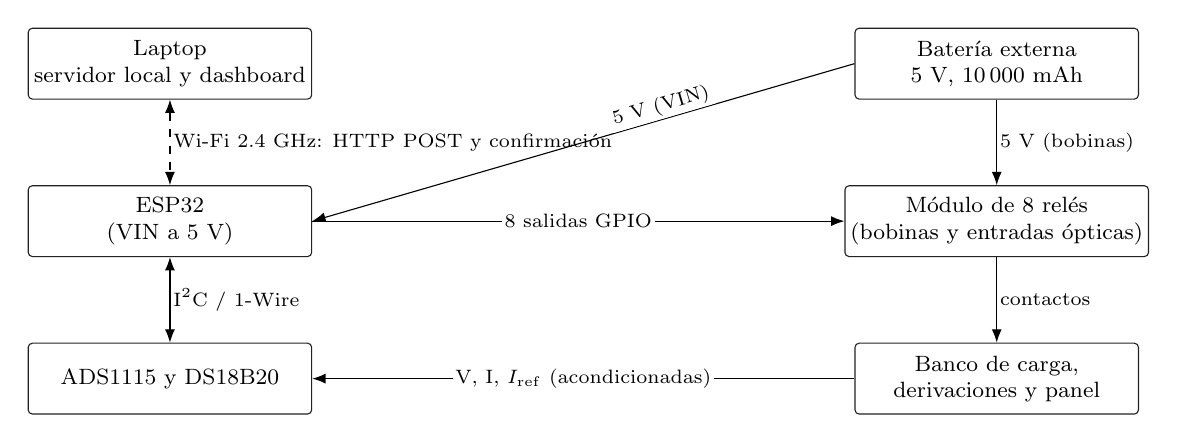
\begin{tikzpicture}[font=\footnotesize,>=Latex,
box/.style={draw=ink,rounded corners=1.5pt,minimum height=0.9cm,minimum width=3.6cm,align=center,inner sep=2pt},
lbl/.style={font=\scriptsize,fill=white,inner sep=1pt}]
\node[box] (pc) at (0,4) {Laptop\\servidor local y dashboard};
\node[box] (pb) at (10.5,4) {Batería externa\\5 V, 10\,000 mAh};
\node[box] (esp) at (0,2) {ESP32\\(VIN a 5 V)};
\node[box] (rel) at (10.5,2) {Módulo de 8 relés\\(bobinas y entradas ópticas)};
\node[box] (sen) at (0,0) {ADS1115 y DS18B20};
\node[box] (car) at (10.5,0) {Banco de carga,\\derivaciones y panel};
\draw[<->,dashed] (pc) -- node[lbl,right]{Wi-Fi 2.4 GHz: HTTP POST y confirmación} (esp);
\draw[->] (pb.west) -- node[lbl,above,sloped,pos=0.35]{5 V (VIN)} (esp.east);
\draw[->] (pb) -- node[lbl,right]{5 V (bobinas)} (rel);
\draw[->] (esp) -- node[lbl]{8 salidas GPIO} (rel);
\draw[<->] (esp) -- node[lbl,right]{I$^2$C / 1-Wire} (sen);
\draw[->] (rel) -- node[lbl,right]{contactos} (car);
\draw[->] (car) -- node[lbl]{V, I, $I_\mathrm{ref}$ (acondicionadas)} (sen);
\end{tikzpicture}
\caption{Arquitectura de alimentación y datos. La batería es la única fuente de 5 V: alimenta al ESP32 y a las bobinas de los relés. La laptop se comunica con el ESP32 solo por Wi-Fi (línea discontinua). La referencia de tierra es común a los bloques conectados por cable.}
\label{fig:arq}
\end{figure*}

Como se ve en la Fig.~\ref{fig:arq}, la batería externa alimenta al ESP32 (por el pin VIN) y a las bobinas del módulo de relés, y la laptop recibe los datos por Wi-Fi. Se descartó dejar las bobinas solas en la batería porque su consumo medio sería de unos 33 mA y muchas baterías se apagan con corrientes bajas; con el ESP32 en el mismo circuito la carga mínima es de unos 130 mA. Las precauciones son:
\begin{itemize}
\item \emph{Una sola fuente de 5 V.} El cable USB solo se conecta para programar o depurar y con la batería desconectada, para evitar dos fuentes de 5 V en paralelo. Con el Wi-Fi, durante los ensayos no hace falta ningún cable entre la placa y la laptop.
\item \emph{Picos.} El pico de 740 mA ocurre solo con todos los relés cerrados y dura menos de 0.3 s; está dentro de la capacidad de la batería.
\item \emph{Apagado automático.} Se probará la batería elegida con la carga real antes de cada sesión de varias horas.
\end{itemize}

% ---------------- IV ----------------
\section{Transmisión y registro de datos}\label{sec:wifi}
\subsection{Medio de transmisión}
Los datos se envían del ESP32 a la laptop por Wi-Fi (2.4~GHz) mediante una petición HTTP POST con contenido JSON a un servidor que se ejecuta en la laptop. El ESP32 no puede usar la dirección \texttt{localhost}, que en el ESP32 se refiere a sí mismo; debe usar la dirección IP de la laptop en la red local. La red puede ser la de un enrutador o un punto de acceso creado por la propia laptop o por un teléfono, siempre en 2.4~GHz, que es la única banda del ESP32; con un punto de acceso propio no se depende del alcance de la red doméstica y la dirección de la laptop es fija. Frente al USB, el Wi-Fi elimina el cable entre la placa y la laptop y la posible alimentación en paralelo de la placa, y permite ver el dashboard desde otro dispositivo de la misma red.

El costo es energético y de ruido: la transmisión eleva el consumo del ESP32 a unos 250 a 280 mA \cite{hubble} y es una fuente de radiofrecuencia y de caída de tensión cerca de las entradas analógicas. Por eso el firmware sigue la regla \emph{medir, luego transmitir}: las lecturas del ADS1115 se hacen siempre fuera de las ráfagas de transmisión, y no se transmite mientras haya relés cerrados. El ESP32 no emplea su convertidor interno, de modo que no hay conflicto con el uso del Wi-Fi. El puerto USB se conserva como respaldo y para depuración, con las mismas líneas CSV.


La Tabla~\ref{tab:med} resume por qué se eligió Wi-Fi frente a las otras opciones.

\begin{table}[t]
\centering
\caption{Alternativas de medio de transmisión}
\label{tab:med}
\footnotesize
\begin{tabular}{@{}p{1.5cm}p{1.8cm}p{3.6cm}@{}}
\toprule
Medio & Hardware extra & Ventajas y desventajas\\
\midrule
USB serie & Ninguno (cable) & Sin pérdidas, pero ata la placa a la laptop y mezcla alimentación y datos\\
Bluetooth LE & Ninguno (integrado) & Bajo consumo; requiere un puente para el servidor y el alcance es corto\\
LoRa & Módulos en ambos extremos & Alcance innecesario aquí; mayor costo y complejidad\\
Wi-Fi 2.4 GHz & Ninguno (integrado) & \textbf{Elegido}: compatible con HTTP/JSON y con el dashboard; mayor consumo\\
\bottomrule
\end{tabular}
\end{table}

\subsection{Servidor local y confiabilidad}
En la laptop se ejecuta un servidor sencillo (Python) con tres funciones: recibir los datos y confirmarlos, guardarlos en un archivo CSV y servir el dashboard. Para no perder datos si la conexión se interrumpe:
\begin{itemize}
\item El ESP32 reúne los puntos de un barrido y los envía en una sola petición al terminar (unos 2.5 kB en JSON), y las lecturas ligeras en peticiones breves. Los barridos no confirmados se conservan en la memoria flash y se reenvían.
\item Cada barrido lleva su \texttt{sweep\_id}; el servidor descarta duplicados y responde con una confirmación que incluye la hora del servidor, con la que el ESP32 sincroniza su reloj sin necesitar internet.
\item Si el servidor no responde, la lectura se marca y se conserva; no se interpola ni se descarta (sección~\ref{sec:faltantes}).
\item Los datos de la red (nombre y contraseña) se guardan en un archivo de configuración fuera del repositorio de código.
\end{itemize}

\subsection{Formato del dato}
Cada punto se registra como un objeto JSON en la transmisión y como una línea de un archivo CSV en la laptop, con las columnas de la Tabla~\ref{tab:csv}. Se guardan los conteos crudos del convertidor además de los valores en unidades físicas, de modo que la calibración (valores reales de resistencias, factor del divisor) pueda reaplicarse después sin perder información. Las magnitudes derivadas (potencia, eficiencia, potencia a 25~\textdegree C e índice de rendimiento) se calculan en la laptop.

\begin{table*}[t]
\centering
\caption{Formato del archivo CSV}
\label{tab:csv}
\footnotesize
\begin{tabularx}{\textwidth}{@{}>{\ttfamily}p{2.6cm}p{1.6cm}X@{}}
\toprule
\normalfont Columna & Unidad & Descripción\\
\midrule
timestamp\_pc & ISO 8601 & Hora de la laptop (UTC$-6$) al recibir el dato.\\
t\_ms & ms & Tiempo del ESP32 desde el arranque, para medir intervalos dentro de un barrido.\\
sweep\_id & --- & Número consecutivo del barrido.\\
pt & --- & Índice del punto (0 corresponde a circuito abierto, todos los relés abiertos).\\
mask & hex & Máscara de 8 bits de los relés cerrados.\\
raw\_v, raw\_i, raw\_ref & cuentas & Lecturas crudas promediadas del ADS1115 (voltaje, corriente del panel, corriente de la celda de referencia).\\
v\_mod & V & Voltaje en los terminales del módulo, con la relación real del divisor.\\
i\_mod & A & Corriente del módulo, con el valor real de la derivación y la corrección de la corriente del divisor.\\
i\_ref & A & Corriente de cortocircuito de la celda de referencia (medida relativa de irradiancia).\\
t\_cell & \textdegree C & Temperatura posterior del módulo; se registra al inicio y al final del barrido.\\
flag & --- & 0: válido; 1: irradiancia inestable; 2: error de lectura o saturación.\\
\bottomrule
\end{tabularx}
\end{table*}

\subsection{Cadencia}
Durante una sesión de ensayo (varias horas) la celda de referencia permanece descubierta, y se cubre al terminar, como establece el protocolo del primer avance. Se propone: una lectura ligera cada 30 s (voltaje de circuito abierto, corriente de la celda de referencia y temperatura) y un barrido completo de la curva cada 10 min. Un barrido de 23 puntos genera unos 1.6 kB en CSV, es decir, unos 10 kB por hora; el almacenamiento no es una restricción. Las lecturas ligeras se transmiten tras cada medición y el barrido, al terminar. La cadencia se ajustará con los resultados de las pruebas.

\subsection{Política de datos faltantes}\label{sec:faltantes}
La cantidad de datos faltantes afecta fuertemente la tasa de degradación estimada, y filtrar los datos corruptos mejora la exactitud de todas las técnicas evaluadas \cite{romero}; la guía de trabajo del curso resume del mismo estudio desviaciones de 0.07 a 0.2\,\%/año con 10\,\% de datos faltantes y de más de 0.6\,\%/año con 50\,\% en valores mensuales \cite{guia}. En consecuencia: (i) nunca se interpolan datos; una lectura inválida se marca con \texttt{flag}\,$\neq 0$ y se conserva; (ii) se reporta el porcentaje de barridos válidos de cada sesión; y (iii) una sesión con menos de 90\,\% de barridos válidos se repite. El umbral de 90\,\% corresponde al nivel de datos faltantes de 10\,\% del estudio citado.

% ---------------- V ----------------
\section{Estrategia de muestreo}\label{sec:muestreo}
\subsection{Configuración del convertidor}
El ADS1115 se opera en modo de disparo único a 475 muestras por segundo (2.1 ms por conversión) \cite{ads1115}. Se leen tres canales por punto: el voltaje en A0 a través del divisor, la corriente del panel de forma diferencial entre A2 y A3 y la corriente de la celda de referencia en A1. En los canales de corriente se usa la escala de $\pm 0.512$ V, que da \SI{15.6}{\micro\volt} por cuenta y, sobre la derivación de \SI{1}{\ohm}, \SI{15.6}{\micro\ampere} \cite{avance1}. Tras cada cambio de canal se descarta la primera conversión y se promedian las ocho siguientes; si el ruido aleatorio no está correlacionado, el promedio lo reduce en $\sqrt{8}\approx 2.8$ veces. El promedio no corrige errores sistemáticos ni deriva, que son competencia de la calibración. La escala del canal de voltaje es de $\pm 4.096$ V (sección~\ref{sec:acond}).

\subsection{Secuencia de un punto}
Para cada punto de la curva: (1) se cierra la combinación de relés; (2) se esperan 200 ms de asentamiento, que superan por amplio margen al filtro de entrada (la constante del divisor con el filtro RC es de unos 0.87 ms, y asentar a una cuenta de 16 bits requiere unas 11 constantes de tiempo, es decir, unos 10 ms); (3) se leen los tres canales en orden corriente, voltaje y referencia, en unos 70 ms; y (4) se abre la combinación. El desfase entre la corriente y el voltaje de un mismo punto es de unas decenas de milisegundos, frente a los minutos que separaron las dos lecturas en la práctica 3 \cite{lab3}, donde la irradiancia cambiaba entre ambas.

\subsection{Duración del barrido y criterio de validez}
Con $N=23$ puntos, seleccionados entre las 256 combinaciones siguiendo \cite{machado}, y un intervalo de $t_\mathrm{int}=5$ s entre puntos, la duración del barrido es
\begin{equation}
T_\mathrm{b}=N\,t_\mathrm{int}+2\,t_T\approx 23\times 5\ \mathrm{s}+2\times 0.75\ \mathrm{s}\approx 117\ \mathrm{s},
\end{equation}
donde $t_T=0.75$ s es el tiempo máximo de conversión del DS18B20 a 12 bits \cite{ds18b20}; la temperatura se lee al inicio y al final y no en cada punto. Si el intervalo se redujera a 2 s, el barrido duraría unos 47 s y el ciclo de trabajo subiría a 13.5\,\%, con una potencia media de unos 0.19 W en la resistencia de 22~$\Omega$ (unos 1.4 W cerrada, según el primer avance), todavía lejos de los 2 W nominales; esa opción se evaluará después de verificar la temperatura de las resistencias en las pruebas.

Como el barrido dura minutos y la irradiancia cambia (práctica 3), la celda de referencia se lee en cada punto. Un barrido se descarta si
\begin{equation}
\rho=\frac{\max(I_\mathrm{ref})-\min(I_\mathrm{ref})}{\overline{I_\mathrm{ref}}}>\rho_\mathrm{max},
\end{equation}
con $\rho_\mathrm{max}=2\,\%$ como valor inicial, que se ajustará con la dispersión medida en cielo estable. Los barridos aceptados pueden normalizarse a una irradiancia común escalando la corriente de cada punto con $I_\mathrm{ref}$; ese procedimiento debe validarse antes de emplearse en el modelo.

\begin{table}[t]
\centering
\caption{Parámetros de muestreo}
\label{tab:muestreo}
\footnotesize
\begin{tabularx}{\columnwidth}{@{}Xr@{}}
\toprule
Parámetro & Valor\\
\midrule
Velocidad del ADS1115 & 475 SPS\\
Muestras promediadas por canal & 8 (más 1 descartada)\\
Escala de los canales de corriente & $\pm 0.512$ V\\
Asentamiento tras cerrar el relé & 200 ms\\
Lectura de los tres canales & $\approx 70$ ms\\
Ciclo de trabajo ($t_\mathrm{int}=5$ s) & 5.4\,\%\\
Puntos por barrido & 23\\
Duración del barrido & $\approx 117$ s\\
Umbral de descarte $\rho_\mathrm{max}$ & 2\,\% (inicial)\\
Barridos válidos requeridos por sesión & $\geq 90$\,\%\\
\bottomrule
\end{tabularx}
\end{table}

% ---------------- II ----------------
\section{Decisión de montaje del módulo}
\subsection{Alternativas consideradas}
Se compararon tres configuraciones, todas para el módulo bajo prueba y su celda de referencia, que deben conservar el mismo plano:
\begin{enumerate}[label=\arabic*)]
\item \emph{Montaje fijo:} inclinación y orientación constantes, sin actuadores.
\item \emph{Giro de base (acimut):} eje vertical que gira el conjunto para seguir el acimut del Sol, con inclinación fija.
\item \emph{Inclinación variable:} eje horizontal orientado norte--sur que inclina el panel de este a oeste siguiendo el recorrido diario del Sol, con la base fija.
\end{enumerate}

\subsection{Evidencia de la literatura}
La Tabla~\ref{tab:lit} resume los estudios consultados. Las cifras provienen de los resúmenes publicados; no se revisaron los textos completos.

\begin{table}[t]
\centering
\caption{Ganancia de energía de los seguidores frente a un montaje fijo}
\label{tab:lit}
\footnotesize
\begin{tabularx}{\columnwidth}{@{}>{\raggedright\arraybackslash}p{0.8cm}>{\raggedright\arraybackslash}p{2.1cm}>{\raggedright\arraybackslash}X@{}}
\toprule
Ref. & Sitio & Resultado\\
\midrule
\cite{lubitz} & 217 sitios de EE.\,UU. (templados) & Acimut: $+29$\,\%; dos ejes: $+34$\,\% frente a fijo con inclinación óptima.\\
\cite{bahrami} & Europa y África & Dos ejes: $+17.7$ a $+31.2$\,\% sobre fijo óptimo; la diferencia entre un eje y dos ejes varía de 0.42 a 23.4\,\% según la latitud.\\
\cite{ordonez} & Quito (ecuatorial) & El eje horizontal es la opción más ventajosa; dos ejes superan a un eje solo marginalmente.\\
\cite{serrano} & Zona tórrida latinoamericana & Un eje: hasta $+23$\,\%; el segundo eje agrega como máximo 4\,\%.\\
\cite{mermoud} & Revisión (PVsyst) & Ganancias de 10 a 50\,\%; el eje horizontal rinde mejor cerca del ecuador.\\
\cite{demirdelen} & Mediterráneo, 15 días & Un eje: $+24.4$\,\%; dos ejes: $+32.2$\,\%.\\
\cite{kibar} & Kocaeli, un año, 2.7 kWp & Un eje: $+28.7$\,\% anual; LCOE 12.2\,\% menor.\\
\bottomrule
\end{tabularx}
\end{table}

En latitudes medias las ganancias se concentran entre 24 y 34\,\%. Cerca del ecuador, donde el Sol pasa próximo al cenit, la literatura coincide en que el eje horizontal es la mejor opción de un eje y en que el segundo eje agrega poco \cite{ordonez,serrano,mermoud}. Esto es relevante porque el giro de base conserva una inclinación fija, y a baja latitud el acimut cambia mucho pero la geometría respecto del Sol cambia poco.

\subsection{Simulación para el sitio}
Para evaluar las tres alternativas en las condiciones de este proyecto se simuló un año completo de irradiancia en el plano del módulo para Antiguo Cuscatlán (13.67° N, 89.25° O, 920 m s.\,n.\,m.). Se empleó la biblioteca pvlib \cite{pvlib}, el modelo de cielo despejado de Ineichen y Perez \cite{ineichen}, la transposición de Hay y Davies \cite{hay}, albedo de 0.2 y paso de 5 min. Los seguidores se modelaron ideales, sin error de seguimiento ni consumo del actuador. La simulación es de cielo despejado y por tanto no incluye nubosidad.

\begin{table}[t]
\centering
\caption{Energía anual incidente simulada (cielo despejado)}
\label{tab:sim}
\footnotesize
\begin{tabular}{@{}p{3.3cm}rrr@{}}
\toprule
Configuración & kWh/m$^2$ & vs 14° S (\%) & vs 30° S (\%)\\
\midrule
Fijo, 14° al sur & 2\,578 & 0 & +3.7 \\
Fijo, 30° al sur (adoptado) & 2\,487 & $-$3.5 & 0 \\
Fijo, 30° al este o al oeste & 2\,280 & $-$11.6 & $-$8.3 \\
Fijo, 30° al norte & 1\,976 & $-$23.4 & $-$20.5 \\
Giro de base (acimut), inclinación 14° & 2\,956 & +14.6 & +18.9 \\
Giro de base (acimut), inclinación 30° & 3\,267 & +26.7 & +31.3 \\
Inclinación este--oeste (eje horizontal N--S) & 3\,339 & +29.5 & +34.2 \\
Dos ejes (referencia) & 3\,527 & +36.8 & +41.8 \\
\bottomrule
\end{tabular}
\end{table}

\begin{figure}[t]
\centering
\includegraphics[width=\columnwidth]{fig_config.pdf}
\caption{Energía anual de cada alternativa frente al montaje fijo a 30° al sur (simulación de cielo despejado, 13.67° N).}
\label{fig:config}
\end{figure}

Los resultados (Tabla~\ref{tab:sim}, Fig.~\ref{fig:config}) son coherentes con la literatura: la inclinación este--oeste ($+34$\,\%) supera ligeramente al giro de base con inclinación de 30° ($+31$\,\%), y el giro de base con la inclinación igual a la latitud (14°) gana solo 19\,\%. También muestran que la orientación importa: a 30° de inclinación, un panel al este o al oeste rinde 8.3\,\% menos que uno al sur, y uno al norte, 20.5\,\% menos.

\begin{figure}[t]
\centering
\includegraphics[width=\columnwidth]{fig_mensual.pdf}
\caption{Energía mensual incidente con inclinación de 14° y de 30°, ambas al sur (simulación de cielo despejado). La zona sombreada indica los meses de los ensayos.}
\label{fig:mensual}
\end{figure}

Respecto de la inclinación fija, 14° (cercana a la latitud) maximiza la energía anual, pero a lo largo del año el óptimo cambia (Fig.~\ref{fig:mensual}). En noviembre y diciembre, que son los meses de los ensayos, 30° entrega 9.1\,\% más que 14° (446 frente a 409 kWh/m$^2$), mientras que en el año completo entrega 3.5\,\% menos. Esto concuerda con la regla de la práctica de laboratorio 3 \cite{lab3}, según la cual el ángulo conveniente en diciembre es del orden de $\varphi+15^\circ\approx 29^\circ$.

\subsection{Energía a escala del módulo y consumo del actuador}
Con el área total de 0.01035~m$^2$ y la eficiencia aparente de 14.5\,\% del primer avance \cite{avance1}, el módulo produciría en promedio unos 10.2 Wh/día a 30° al sur en cielo despejado, y la inclinación este--oeste lo elevaría a unos 13.7 Wh/día: una ganancia de unos 3.5 Wh/día. Es una estimación idealizada, pero basta para el argumento de escala.

La ganancia es comparable con el consumo posible del actuador. En un experimento de aficionado con un seguidor pequeño \cite{switchdoc}, el motor con sus devanados energizados consumía unos 170 mA, es decir, unos 11 Wh/día de operar de forma continua frente a unos 4 Wh/día de ganancia; solo resultaba rentable con un ciclo de trabajo muy bajo (unos 2 s de cada 360 s). La fuente no está revisada por pares y no se presenta como evidencia cuantitativa general, sino como una ilustración del orden de magnitud. En un módulo de 1.5 W, un motor paso a paso de mayor tamaño exigiría además un controlador y una fuente propios, de modo que el seguimiento solo tendría ganancia neta con una gestión cuidadosa de la energía del actuador.

\subsection{Efecto sobre la medición}
El objetivo del proyecto es detectar degradación, no maximizar la energía. Un módulo móvil agrega fuentes de variación que el sistema fijo no tiene:
\begin{itemize}
\item \emph{Ángulo de incidencia variable.} El índice de rendimiento (ec.~3 del primer avance) usa la corriente de la celda de referencia como medida de irradiancia; esto solo es válido si ambos módulos comparten plano y ángulo. Con un montaje fijo, esa condición se cumple por construcción.
\item \emph{Error de seguimiento.} En \cite{switchdoc} se midió un desalineamiento de 12° a 16° con el seguidor en operación.
\item \emph{Ruido eléctrico del actuador.} Las corrientes de interés son de decenas de miliamperios con resolución de \SI{15.6}{\micro\ampere}; un motor y su controlador en la misma alimentación son una fuente de perturbación que habría que caracterizar.
\item \emph{Cableado móvil y fatiga mecánica.} Aumenta el riesgo de contactos intermitentes, que se confundirían con aumento de resistencia serie, el mismo mecanismo que se desea diagnosticar.
\end{itemize}
Con un montaje fijo, un error geométrico constante se cancela en el índice, que se normaliza contra el estado inicial del propio módulo (ec.~3 de \cite{avance1}), de modo que la diferencia de 3.5\,\% anual respecto del óptimo geométrico no afecta la detección de tendencias.

\subsection{Comparación y configuración adoptada}
\begin{table*}[t]
\centering
\caption{Comparación de las alternativas de montaje}
\label{tab:comp}
\footnotesize
\begin{tabularx}{\textwidth}{@{}>{\raggedright\arraybackslash}p{3.0cm}XXX@{}}
\toprule
Criterio & Fijo & Giro de base (acimut) & Inclinación este--oeste\\
\midrule
Ganancia anual frente al fijo 30° S (simulada) & Referencia & $+31$\,\% (inclinación de 30°) & $+34$\,\%\\
Consumo del actuador & Ninguno & Motor y controlador & Motor y controlador\\
Ganancia neta tras el actuador & --- & Positiva solo con ciclo de trabajo muy bajo \cite{switchdoc} & Ídem\\
Elementos adicionales & Ninguno & Motor, controlador, fuente, base giratoria y referencia de posición & Motor, controlador, fuente, eje y referencia de posición\\
Complejidad mecánica & Baja & Alta (eje vertical con panel inclinado, carga de viento) & Media--alta\\
Complejidad de firmware & Ninguna & Control de posición y cálculo solar & Ídem\\
Efecto sobre la medición & Plano y ángulo constantes; referencia coplanar & Ángulo variable, error de seguimiento, cableado móvil, ruido del actuador & Ídem\\
Fiabilidad a la intemperie & Alta & Media & Media\\
Riesgo de plazo (prototipo funcional: 26 a 30 de octubre) & Ninguno & Alto & Alto\\
\bottomrule
\end{tabularx}
\end{table*}

La Tabla~\ref{tab:comp} resume la comparación. Se adopta el \textbf{montaje fijo con inclinación de 30° y orientación al sur geográfico (azimut de 180°)}, por cuatro razones: (i) en la ventana de ensayos rinde 9\,\% más que a 14° (Fig.~\ref{fig:mensual}); (ii) en la práctica 3 la potencia varió menos de 7\,\% entre 0° y 60° de inclinación y se recomendó 30° con orientación al sur \cite{lab3}; (iii) preserva la comparabilidad del índice de rendimiento y de la celda de referencia; y (iv) no añade consumo, componentes ni riesgo de plazo. La inclinación y el azimut se fijarán con nivel y brújula y se documentarán fotográficamente. El seguimiento queda como trabajo futuro, con la comparación de este apartado como punto de partida.

% ---------------- VII ----------------
\section{Esquemático y lista de componentes}\label{sec:esq}
\subsection{Esquemático del circuito de adquisición}
El esquemático (Fig.~\ref{fig:esq}; completo, en tamaño A3, en el Anexo~A) reúne el ESP32 (U1), el ADS1115 (U2), el DS18B20 (U3), el panel de prueba (J1) y el de referencia (J4), las dos derivaciones de \SI{1}{\ohm} (R\_sh1 y R\_sh2), el divisor R1--R2 con el filtro R3--C1, y el banco de ocho relés (K1 a K8) con sus resistencias de carga RL1 a RL8, gobernados desde el conector J2 del módulo de relés. La hoja incluye también la alimentación (batería externa J5 de 5 V, con el capacitor C4 de \SI{10}{\micro\farad}, hacia VIN del ESP32 y hacia la alimentación del módulo de relés), las resistencias de subida R6 y R7 (4.7 k$\Omega$) del bus I$^2$C, y el modelo del módulo (fuente de corriente V1 de 0.212 A con el diodo D1) usado en la simulación. La Tabla~\ref{tab:conex} resume las conexiones y la Tabla~\ref{tab:bom}, los componentes y su costo.

\begin{figure*}[!t]
\centering
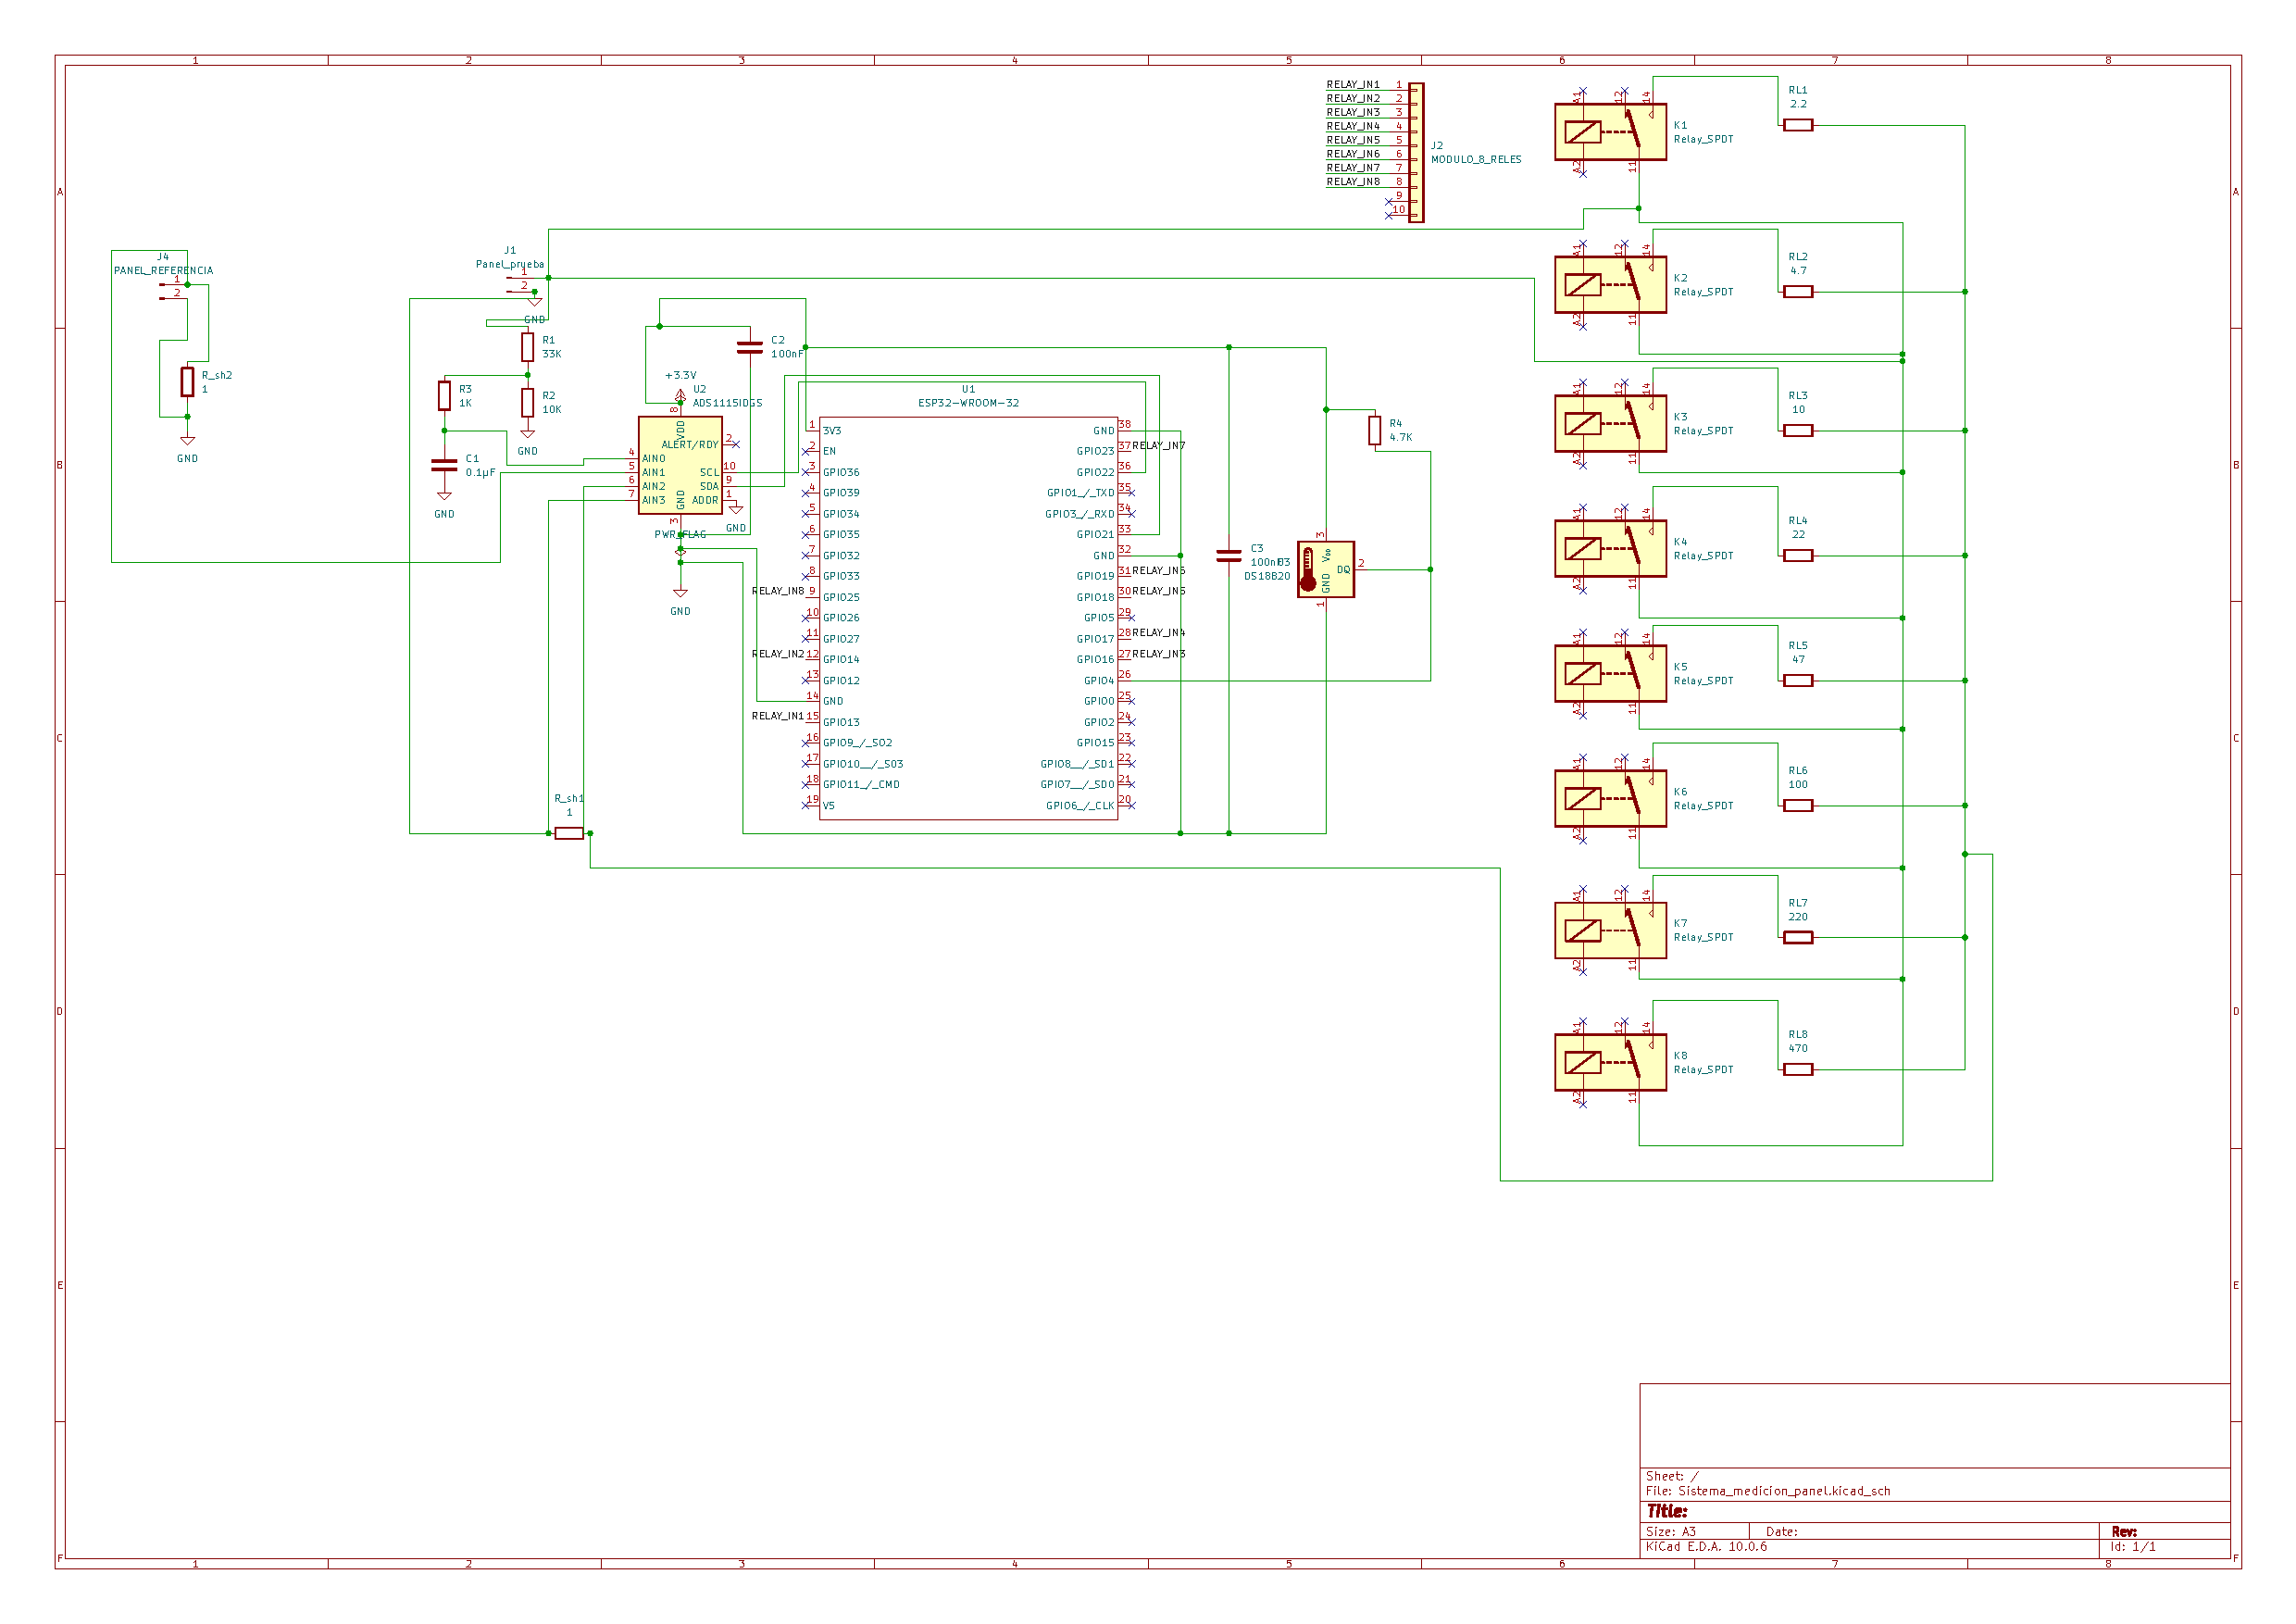
\includegraphics[trim=45pt 387pt 380pt 45pt,clip,width=\textwidth]{Sistema_medicion_panel.pdf}
\caption{Esquemático del circuito de adquisición (detalle del acondicionamiento de señal, el ESP32 y los sensores; el banco de relés y cargas se muestra completo en el Anexo~A). Generado en KiCad.}
\label{fig:esq}
\end{figure*}

\begin{table*}[!t]
\centering
\caption{Conexiones del circuito de adquisición}
\label{tab:conex}
\footnotesize
\begin{tabularx}{\textwidth}{@{}p{3.3cm}p{3.6cm}X@{}}
\toprule
Función & Nodo del esquemático & Conexión\\
\midrule
Bus I$^2$C & U2: SDA (pin 9), SCL (pin 10) & GPIO21 (SDA) y GPIO22 (SCL); ADDR a GND\\
Voltaje del módulo & U2: AIN0 & Divisor R1 (33 k$\Omega$) y R2 (10 k$\Omega$), con filtro R3 (1 k$\Omega$) y C1 (0.1 $\mu$F)\\
Corriente de la celda de referencia & U2: AIN1 & Derivación R\_sh2 (1 $\Omega$), panel de referencia J4\\
Corriente del módulo & U2: AIN2--AIN3 (diferencial) & Derivación R\_sh1 (1 $\Omega$) en serie con la carga, panel de prueba J1\\
Temperatura & U3: DQ & GPIO4, con resistencia de subida R4 (4.7 k$\Omega$) a 3.3 V y C3 (0.1 $\mu$F)\\
Control de relés & J2: RELAY\_IN1 a IN8 & GPIO13, 14, 16, 17, 18, 19, 23 y 25, respectivamente\\
Cargas & K1 a K8 con RL1 a RL8 & 2.2, 4.7, 10, 22, 47, 100, 220 y 470 $\Omega$\\
Desacople & C2 & 0.1 $\mu$F en la alimentación (VDD) de U2\\
Alimentación & J5 (batería 5 V), C4 & +5 V a VIN de U1 y a la alimentación de J2 (pines 9 y 10); +3.3 V del regulador de U1 a U2, R4, R6 y R7\\
Pull-ups I$^2$C & R6, R7 & 4.7 k$\Omega$ de SDA y SCL a +3.3 V\\
\bottomrule
\end{tabularx}
\end{table*}

\subsection{Lista de componentes y costo}
La Tabla~\ref{tab:bom} reproduce la lista del primer avance \cite{avance1}, con los precios de las cotizaciones de Casa Rivas (CR; con 25 \% de descuento estudiantil y IVA) y de Steren (con IVA), y la referencia de cada componente en el esquemático. El total a adquirir es de USD 32.57. La batería externa ya era propiedad del equipo y no se compró para este proyecto; se incluye con un valor de referencia de USD 20.00, de modo que el costo total del proyecto es de USD 52.57.

\begin{table*}[!t]
\centering
\caption{Lista de componentes y costo}
\label{tab:bom}
\footnotesize
\begin{tabularx}{\textwidth}{@{}p{1.9cm}Xcrrl@{}}
\toprule
Ref. & Componente & Cant. & P. unit. (USD) & Subtotal (USD) & Fuente\\
\midrule
J1, J4 & Módulo fotovoltaico 5 V / 1.5 W, AR-3302PANEL5V (prueba y referencia) & 2 & 6.95 & 13.90 & CR\\
U2 & Convertidor ADS1115, AR-ADS1115 & 1 & 3.71 & 3.71 & CR\\
U3 & Sonda DS18B20, AR-DS18B20A & 1 & 2.06 & 2.06 & CR\\
J2, K1--K8 & Módulo de 8 relés optoacoplado & 1 & 4.50 & 4.50 & Steren\\
R\_sh1, R\_sh2 & Derivación 1 $\Omega$ / 1 W, película metálica & 2 & 0.60 & 1.20 & Steren\\
R1 & Resistencia 33 k$\Omega$ (divisor) & 1 & 0.30 & 0.30 & Steren\\
R2 & Resistencia 10 k$\Omega$, KD10N0.5 (divisor) & 1 & 0.15 & 0.15 & CR\\
R4, R6, R7 & Resistencia 4.7 k$\Omega$ (1-Wire y subida de I$^2$C) & 3 & 0.30 & 0.90 & Steren\\
R3 & Resistencia 1 k$\Omega$ (filtro RC) & 1 & 0.30 & 0.30 & Steren\\
C1--C3 & Capacitor cerámico 0.1 $\mu$F & 3 & 0.10 & 0.30 & Steren\\
C4 & Capacitor 10 $\mu$F (alimentación de 5 V) & 1 & 0.25 & 0.25 & CR\\
RL1--RL6 & Banco de carga 2 W: 2.2, 4.7, 10, 22, 47 y 100 $\Omega$ & 6 & 0.40 & 2.40 & Steren\\
RL7, RL8 & Banco de carga 1/2 W: 220 y 470 $\Omega$ & 2 & 0.30 & 0.60 & Steren\\
--- & Cinta de aluminio (fijación térmica) & 1 & 2.00 & 2.00 & Steren\\
\midrule
\multicolumn{4}{@{}l}{\textbf{Total a adquirir}} & \textbf{32.57} & \\
\midrule
U1 & ESP32-WROOM-32 & 1 & --- & --- & Disponible\\
--- & Protoboard, conductores, multímetro y cautín & --- & --- & --- & Disponible\\
J5 & Batería externa 5 V, 10\,000 mAh (sección~\ref{sec:alim}); ya era propiedad del equipo, valor de referencia & 1 & 20.00 & 20.00 & Disponible\\
\midrule
\multicolumn{4}{@{}l}{\textbf{Costo total del proyecto (con el valor de la batería)}} & \textbf{52.57} & \\
\bottomrule
\end{tabularx}
\end{table*}

% ---------------- VIII ----------------
\section{Diseño del dashboard}\label{sec:dash}
\subsection{Objetivo y usuario}
El dashboard es la interfaz de quien opera la instalación y debe decidir si limpiar o revisar el módulo. Por eso se ordena de lo urgente a lo detallado: arriba, el estado de mantenimiento; después, las magnitudes del último barrido en tarjetas con unidades; luego las curvas I-V y P-V con la curva esperada de un módulo nuevo; y al final, la evolución del día y el histórico de 30 días (Figs.~\ref{fig:dash1} y \ref{fig:dash2}). Es una sola página HTML sin dependencias, que se abre en el navegador de la laptop, con tema claro y oscuro y exportación del barrido a CSV.

\subsection{Datos y funcionamiento}
Recibe los datos del servidor local (sección~\ref{sec:wifi}) como mensajes JSON por WebSocket o por consulta HTTP: inicio de barrido, puntos de tensión y corriente, y fin de barrido con la temperatura y la irradiancia. De los puntos de cada barrido calcula la potencia máxima, $V_\mathrm{oc}$, $I_\mathrm{sc}$ y el factor de forma, y de ahí las magnitudes derivadas de la Tabla~\ref{tab:ind}. Mientras no esté el hardware, un modo de simulación genera barridos con un modelo de diodo único (15 celdas en serie, $V_\mathrm{oc}=9$ V a 25~°C y 1000 W/m$^2$, 1.5 W) y cinco escenarios: panel limpio, suciedad moderada, suciedad severa, nube pasajera y día caluroso. Todas las cifras de las figuras provienen de esa simulación y no son mediciones.

\begin{table*}[!t]
\centering
\caption{Indicadores del dashboard y su justificación}
\label{tab:ind}
\footnotesize
\begin{tabularx}{\textwidth}{@{}p{3.2cm}p{5.4cm}X@{}}
\toprule
Indicador & Cálculo & Por qué se muestra\\
\midrule
$V$, $I$ y $P$ en el punto de máxima potencia & Del barrido de 23 puntos; $P=VI$ & Variables primarias; muestran el punto de operación y alimentan todo lo demás\\
Temperatura de celda & DS18B20 sobre el módulo & La potencia cae unos 0.4 \%/°C; separa la pérdida térmica reversible de la degradación\\
Irradiancia $G$ & Celda de referencia coplanar (corriente de cortocircuito relativa) & Normaliza la potencia; sin ella no se distingue una nube de suciedad\\
Eficiencia real contra nominal & $\eta=P/(G\,A)$, con $A=0.01035$ m$^2$; nominal 14.5 \% (1.5 W en 1000 W/m$^2$) & Compara el rendimiento del módulo con su placa\\
Índice de rendimiento (PR) corregido por temperatura & $\mathrm{PR}=P\,/\,[P_\mathrm{nom}(G/1000)(1+\gamma(T-25))]$ & Índice de la norma IEC 61724-1 independiente del clima; es la señal central del modelo de degradación\\
Potencia a STC y degradación & $P_\mathrm{STC}=P/[(G/1000)(1+\gamma\Delta T)]$; $D=(P_\mathrm{nom}-P_\mathrm{STC})/P_\mathrm{nom}$ & Estimación en porcentaje, comparable con la placa\\
Factor de forma, $V_\mathrm{oc}$ e $I_\mathrm{sc}$ contra lo esperado & $\mathrm{FF}=P/(V_\mathrm{oc}I_\mathrm{sc})$; desviación respecto de la curva de un módulo nuevo en las mismas $G$ y $T$ & La degradación afecta distinto a cada parámetro (en el primer avance, el factor de forma cae más que $I_\mathrm{sc}$ y casi no cambia $V_\mathrm{oc}$) \cite{avance1}; permite diagnosticar la causa\\
Curvas I-V y P-V & Puntos medidos y modelo de diodo & Evidencia visual del barrido y del punto de máxima potencia\\
PR diario (30 días) y umbral & Cociente de sumas diarias, solo con $G\ge 200$ W/m$^2$ & Tendencia de largo plazo que filtra el ruido de las nubes\\
Alerta de mantenimiento & Regla de la subsección~\ref{sec:alerta} & Convierte la tendencia en una acción para el usuario\\
\bottomrule
\end{tabularx}
\end{table*}

\subsection{Alerta de mantenimiento}\label{sec:alerta}
El PR diario se calcula como cociente de sumas,
\begin{equation}
\mathrm{PR}_d=\frac{\sum P_\mathrm{max}}{\sum P_\mathrm{nom}\,(G/1000)\,[1+\gamma(T-25)]},
\end{equation}
solo con los barridos de $G\ge\SI{200}{\watt\per\meter\squared}$, como en la norma IEC 61724-1. El estado es \emph{normal} sobre el umbral, \emph{vigilar} con uno o dos días seguidos bajo el umbral, y \emph{mantenimiento recomendado} con tres. Exigir tres días evita alertar por jornadas nubladas aisladas. El umbral inicial es de 90 \% y es editable: la degradación permanente descrita en el primer avance es de menos de 1 \% al año \cite{avance1}, de modo que una caída de 10 \% en pocas semanas apunta a causas reversibles, sobre todo suciedad.

La alerta incluye un diagnóstico probable a partir de la última curva: si $I_\mathrm{sc}$ cae más de 7 \% respecto de lo esperado con el factor de forma normal, se sugiere suciedad o sombreado parcial; si el factor de forma cae más de 8 \%, resistencia serie alta o conexiones deterioradas; y en otro caso, pérdida repartida compatible con envejecimiento. Estas reglas y el umbral son valores iniciales, que se calibrarán con la línea base del módulo limpio.

\begin{figure*}[!t]
\centering
\includegraphics[width=\textwidth]{dash_top.png}
\caption{Prototipo del dashboard, parte superior: estado de mantenimiento, magnitudes del último barrido, curvas I-V y P-V medidas frente a las esperadas, y diagnóstico del panel. Escenario de suciedad moderada con datos simulados.}
\label{fig:dash1}
\end{figure*}

\begin{figure*}[!t]
\centering
\includegraphics[width=\textwidth]{dash_bot.png}
\caption{Prototipo del dashboard, parte inferior: potencia, irradiancia y temperatura del día; eficiencia real contra nominal; alerta de mantenimiento; PR diario de 30 días con el umbral; y registro del barrido. Datos simulados.}
\label{fig:dash2}
\end{figure*}

\subsection{Interpretación del prototipo}
En el escenario de suciedad moderada, el barrido de las 14:50 (irradiancia de 664 W/m$^2$, temperatura de celda de 46.3~°C) entrega \SI{0.79}{\watt} frente a \SI{0.89}{\watt} esperados (\SI{-11.2}{\percent}). La pérdida se concentra en la corriente ($I_\mathrm{sc}$ de \SI{-11.0}{\percent}) y no en el voltaje ($V_\mathrm{oc}$ de \SI{0.0}{\percent}) ni en la forma de la curva (factor de forma de \SI{-0.2}{\percent}). La eficiencia es de 11.5 \% frente a 14.5 \% nominal, el PR diario es de 88.2 \% y el histórico lleva seis días bajo el umbral, por lo que se activa la alerta y el diagnóstico apunta a suciedad. Como la degradación del escenario está programada en la simulación, este resultado solo comprueba que los indicadores distinguen la causa; no valida el modelo con datos reales.

\subsection{Alcance actual}
El dashboard funciona con datos simulados. Falta conectarlo al servidor local con barridos reales del ESP32 y calibrar las reglas de alerta con la línea base del módulo limpio.

% ---------------- IX ----------------
\section{Simulación o pruebas físicas}\label{sec:sim}
Esta sección presenta la simulación del circuito de adquisición. Primero se resumen los valores teóricos de referencia (Tabla~\ref{tab:teor}), que resultan de los divisores y escalas de la sección~\ref{sec:acond}, y luego se contrastan con los resultados simulados.

\begin{table}[t]
\centering
\caption{Valores teóricos de referencia para la simulación}
\label{tab:teor}
\footnotesize
\begin{tabular}{@{}lccr@{}}
\toprule
Magnitud & Valor & Tensión en el ADC & Cuentas\\
\midrule
$V_\mathrm{oc}$ & 9.0 V & 2.093 V (A0) & 16\,744\\
$V_\mathrm{mp}$ & 7.5 V & 1.744 V (A0) & 13\,954\\
$I_\mathrm{sc}$ & 0.212 A & 0.212 V (A2--A3) & 13\,568\\
$I_\mathrm{mp}$ & 0.200 A & 0.200 V (A2--A3) & 12\,800\\
\bottomrule
\end{tabular}

\smallskip
{\scriptsize Escalas de $\pm 4.096$ V (cuenta de 125 $\mu$V) en A0 y de $\pm 0.512$ V (15.625 $\mu$V) en A2--A3. $I_\mathrm{sc}$, $V_\mathrm{mp}$ e $I_\mathrm{mp}$ son estimaciones coherentes con 1.5 W.}
\end{table}

\subsection{Modelo y método}
La simulación se ejecutó con ngspice (el motor del simulador de KiCad 10) sobre el circuito de adquisición de la sección~\ref{sec:esq}: el divisor R1 (33 k$\Omega$) y R2 (10 k$\Omega$), el filtro R3 (1 k$\Omega$) y C1 (0.1 $\mu$F) hacia A0, la derivación R\_sh1 de 1 $\Omega$ hacia A2--A3 y el banco de cargas de 2.2 a 470 $\Omega$, con cada relé modelado como un interruptor con resistencia de contacto de 50 m$\Omega$. El módulo se modeló como una fuente de corriente (fotocorriente de 0.212 A) en paralelo con un diodo (corriente de saturación de 3.74 nA y factor $N=19.5$, es decir, 15 celdas en serie con factor de idealidad de 1.3), lo que da $V_\mathrm{oc}=9.0$ V, $I_\mathrm{sc}=0.212$ A y $P_\mathrm{max}=1.51$ W a 7.6 V y 0.199 A (factor de forma de 0.79). Las entradas del ADS1115 se modelaron como 5 M$\Omega$ a tierra (valor supuesto, del orden de lo que indica la hoja de datos \cite{ads1115}). Estos parámetros del módulo son estimaciones coherentes con 1.5 W y con el $V_\mathrm{oc}$ de 9 V, no mediciones. Las lecturas del ADS1115 se obtuvieron redondeando a la cuenta más cercana (125 $\mu$V en A0 y 15.625 $\mu$V en A2--A3).

Se simularon cinco cosas: (i) la curva I-V y P-V del módulo; (ii) el barrido de 23 puntos con el circuito completo, con las 255 combinaciones de relés disponibles y la selección descrita abajo; (iii) el transitorio al cerrar un relé; (iv) el mismo barrido con una pérdida de 11 \% en la fotocorriente, que emula suciedad; y (v) escenarios de irradiancia y temperatura (subsección siguiente a los resultados).

\subsection{Selección de los 23 puntos}
Con las 255 combinaciones de cargas en paralelo se calculó el punto de operación de cada una. Para repartir los puntos de forma pareja a lo largo de la curva se tomó el circuito abierto y, de las demás combinaciones, las 22 más próximas a puntos equidistantes en longitud de arco de la curva I-V normalizada ($V/V_\mathrm{oc}$, $I/I_\mathrm{sc}$). Las máscaras resultantes (en hexadecimal, con el bit 0 en RL1 y el bit 7 en RL8) son, de menor a mayor voltaje: 01, 3C, A4, 78, E8, C8, 08, F0, 70, B0, 30, D0, 50, 90, 10, E0, 60, A0, 20, C0, 40, 80 y 00 (circuito abierto). Esta selección es una propuesta de la simulación y debe confirmarse con el módulo real, cuya curva puede diferir.

\subsection{Resultados}
\begin{figure}[t]
\centering
\includegraphics[width=\columnwidth]{fig_sim_iv.pdf}
\caption{Curvas I-V y P-V simuladas del módulo (línea continua: limpio; discontinua: con 11 \% menos de fotocorriente) y los 23 puntos del barrido con el circuito completo (círculos).}
\label{fig:simiv}
\end{figure}

La Fig.~\ref{fig:simiv} muestra que los 23 puntos caen sobre la curva del módulo y cubren tanto la zona plana como el codo. La Tabla~\ref{tab:simres} resume algunos puntos. Los resultados son:
\begin{itemize}
\item \emph{Escalas.} En circuito abierto A0 recibe 2.090 V (16\,723 cuentas), 0.1 \% por debajo de los 2.093 V teóricos de la Tabla~\ref{tab:teor}; la diferencia la explica el efecto de carga de la entrada del ADS1115. Con 11 V (máximo de diseño) serían 2.56 V, lejos de los 4.096 V de la escala. En la derivación, la corriente de cortocircuito produce 0.212 V (13\,567 cuentas), 41 \% de la escala de 0.512 V, con un margen de 2.4 veces.
\item \emph{Punto de máxima potencia.} El barrido encuentra 1.5075 W con la combinación de 35.8 $\Omega$ (máscara D0), frente a 1.512 W de la curva exacta (diferencia de 0.3 \%). Tras convertir las cuentas a voltios y amperios, la potencia estimada es de 1.5049 W, un error de $-0.17$ \% que proviene de la carga de la entrada del ADS1115 sobre el divisor y que se corrige con la calibración.
\item \emph{Corriente del divisor.} El divisor consume $V/43$ k$\Omega$ ($\approx 0.2$ mA en circuito abierto), que no pasa por la derivación; la corriente del módulo es la de la derivación más esa corriente, una diferencia de 0.1 \% que el cálculo debe incluir.
\item \emph{Suciedad.} Con 11 \% menos de fotocorriente, la potencia máxima del barrido cae a 1.333 W ($-11.6$ \%), la corriente de cortocircuito en la derivación baja de 212 a 189 mV y el voltaje de circuito abierto casi no cambia (8.945 V frente a 9.004 V). Es el patrón que el dashboard usa para sugerir suciedad.
\end{itemize}

\begin{table}[t]
\centering
\caption{Puntos del barrido simulado (valores de A0 y A2--A3 con sus cuentas)}
\label{tab:simres}
\footnotesize
\begin{tabular}{@{}rcccrr@{}}
\toprule
$R_\mathrm{eq}$ ($\Omega$) & Máscara & $V$ (V) & A0 (V) & Derivación (mV) & $P$ (W)\\
\midrule
$\infty$ & 00 & 9.00 & 2.090 (16\,723) & 0.0 (0) & 0.000\\
2.2 & 01 & 0.69 & 0.160 (1\,280) & 212.0 (13\,567) & 0.146\\
8.9 & A4 & 2.11 & 0.490 (3\,920) & 212.0 (13\,565) & 0.447\\
22.0 & 08 & 4.88 & 1.134 (9\,068) & 211.8 (13\,557) & 1.034\\
32.0 & 30 & 6.89 & 1.599 (12\,789) & 208.7 (13\,354) & 1.437\\
35.8 & D0 & 7.45 & 1.729 (13\,835) & 202.4 (12\,952) & 1.507\\
42.7 & 90 & 8.00 & 1.858 (14\,861) & 182.8 (11\,700) & 1.463\\
68.8 & 60 & 8.57 & 1.989 (15\,911) & 122.8 (7\,858) & 1.052\\
149.9 & C0 & 8.84 & 2.053 (16\,420) & 58.6 (3\,750) & 0.518\\
470.0 & 80 & 8.96 & 2.080 (16\,638) & 19.0 (1\,217) & 0.170\\
\bottomrule
\end{tabular}
\end{table}

\subsection{Escenarios de irradiancia y temperatura}
Para el rubro de escenarios se repitió el barrido de 23 puntos con el circuito completo variando la irradiancia $G$ (200 a 1\,100 W/m$^2$ a 25 \textdegree C) y la temperatura del módulo (15, 45 y 65 \textdegree C a 1\,000 W/m$^2$, más dos combinaciones intermedias). La fotocorriente se escaló como $I_\mathrm{ph}=0.212\,(G/1000)\,[1+0.0005\,(T-25)]$ (coeficiente de $I_\mathrm{sc}$ de $+0.05$ \%/\textdegree C, valor típico del silicio, supuesto) y la dependencia del diodo con la temperatura la calcula ngspice con $E_g$ de 15 celdas (16.8 eV); la corriente de saturación se recalibró (3.32 nA a 25 \textdegree C) para que $V_\mathrm{oc}$ sea 9.0 V a 1\,000 W/m$^2$ y 25 \textdegree C. Con ese modelo $P_\mathrm{max}$ cae 0.40 \%/\textdegree C y $V_\mathrm{oc}$ unos 30 mV/\textdegree C, órdenes de magnitud típicos de un módulo de silicio cristalino, pero siguen siendo supuestos hasta medir el módulo. La Tabla~\ref{tab:simesc} y la Fig.~\ref{fig:simesc} resumen los resultados.

\begin{figure}[t]
\centering
\includegraphics[width=\columnwidth]{fig_sim_esc.pdf}
\caption{Potencia máxima teórica (curva exacta del modelo) y obtenida con el barrido de 23 puntos tras la cuantización, en función de la irradiancia (izquierda, 25 \textdegree C) y de la temperatura (derecha, 1\,000 W/m$^2$).}
\label{fig:simesc}
\end{figure}

\begin{table}[t]
\centering
\caption{Escenarios simulados: teoría (curva exacta del modelo) frente al barrido con el circuito completo y las lecturas máximas en los canales}
\label{tab:simesc}
\scriptsize
\setlength{\tabcolsep}{2.6pt}
\begin{tabular}{@{}rrrrrrrrr@{}}
\toprule
$G$ & $T$ & $V_\mathrm{oc}$ & $I_\mathrm{sc}$ & $P_\mathrm{teo}$ & $P_\mathrm{med}$ & Dif. & A0 máx. & Deriv.\ máx.\\
(W/m$^2$) & (\textdegree C) & (V) & (mA) & (W) & (W) & (\%) & (V) & (mV)\\
\midrule
200 & 25 & 8.20 & 42 & 0.271 & 0.258 & -4.7 & 1.90 & 42\\
400 & 25 & 8.54 & 85 & 0.569 & 0.559 & -1.7 & 1.98 & 85\\
600 & 25 & 8.74 & 127 & 0.878 & 0.875 & -0.3 & 2.03 & 127\\
800 & 25 & 8.89 & 170 & 1.193 & 1.190 & -0.3 & 2.06 & 170\\
1000 & 25 & 9.00 & 212 & 1.513 & 1.507 & -0.5 & 2.09 & 212\\
1100 & 25 & 9.05 & 233 & 1.675 & 1.663 & -0.7 & 2.10 & 233\\
1000 & 15 & 9.30 & 211 & 1.574 & 1.572 & -0.1 & 2.16 & 211\\
1000 & 45 & 8.40 & 214 & 1.391 & 1.383 & -0.6 & 1.95 & 214\\
1000 & 65 & 7.80 & 216 & 1.267 & 1.263 & -0.3 & 1.81 & 216\\
800 & 45 & 8.29 & 171 & 1.094 & 1.091 & -0.3 & 1.92 & 171\\
600 & 15 & 9.05 & 127 & 0.915 & 0.905 & -1.1 & 2.10 & 127\\
\bottomrule
\end{tabular}
\end{table}

\begin{itemize}
\item \emph{Rangos.} En todos los escenarios A0 queda entre 1.8 y 2.2 V (límite de 4.096 V) y la derivación entre 42 y 233 mV (límite de 0.512 V), es decir, las lecturas de $V$ e $I$ quedan dentro de rango y sin saturar; con 15 \textdegree C y 1\,100 W/m$^2$ (el caso extremo del sitio) el máximo de A0 sería de unos 2.2 V.
\item \emph{Irradiancia.} La celda de referencia (A1, derivación de 1 $\Omega$ y escala de $\pm 0.512$ V) entrega 42 a 233 mV si se supone una celda con la misma $I_\mathrm{sc}$ que el módulo, con un margen de 2.2 veces en el máximo y una resolución de 15.6 $\mu$V, equivalente a 0.07 W/m$^2$; el valor real depende de la celda que se adquiera y la relación $G$--tensión debe calibrarse con un piranómetro o con la hoja del fabricante.
\item \emph{Temperatura.} El sensor DS18B20 \cite{ds18b20} cubre de $-55$ a 125 \textdegree C, con $\pm 0.5$ \textdegree C entre $-10$ y 85 \textdegree C, de modo que los 15 a 65 \textdegree C simulados quedan dentro de su rango y de su zona de mejor exactitud; con el coeficiente de $-0.40$ \%/\textdegree C, un error de 0.5 \textdegree C equivale a 0.2 \% en la potencia corregida.
\item \emph{Contraste con la teoría.} A 1\,000 W/m$^2$ la potencia del barrido difiere de la teórica en $-0.4$ \% (25 \textdegree C) y $-0.3$ a $-0.6$ \% (15 a 65 \textdegree C), dentro de la incertidumbre esperada; la diferencia crece al bajar la irradiancia, hasta $-5$ \% a 200 W/m$^2$, porque los 23 puntos se eligieron para la curva de 1\,000 W/m$^2$ y con poca luz el codo se desplaza y queda entre dos puntos.
\end{itemize}

\subsection{Ajustes de diseño derivados de la simulación}
\begin{itemize}
\item Con 400 W/m$^2$ o menos el error del barrido supera 1.5 \%; el firmware debe refinar el barrido alrededor del máximo (agregar combinaciones de relés cercanas al punto de mayor potencia) o descartar esas mediciones para el índice de rendimiento. Se adopta lo segundo como regla por defecto: el índice solo se calcula con $G\ge 600$ W/m$^2$.
\item El error de $-0.17$ \% por la carga de la entrada del ADS1115 se corrige con una calibración de la ganancia del divisor medida con el multímetro.
\item La derivación de 1 $\Omega$ usa solo el 41 \% de su escala a 1\,000 W/m$^2$, por lo que se mantiene la escala de $\pm 0.512$ V; usar una derivación mayor mejoraría la resolución, pero la caída de 0.2 V sobre ella reduciría la potencia del módulo medida.
\item Se mantiene el tiempo de espera de 200 ms por punto, y se agrega una lectura de A1 y de temperatura antes y después de cada barrido para descartar los barridos con irradiancia inestable.
\end{itemize}

\subsection{Asentamiento}
\begin{figure}[t]
\centering
\includegraphics[width=\columnwidth]{fig_sim_tr.pdf}
\caption{Voltaje en A0 al cerrar el relé de 22 $\Omega$ (el panel pasa de circuito abierto a carga). El valor final es 1.134 V.}
\label{fig:simtr}
\end{figure}
Al cerrar el relé de 22 $\Omega$, A0 pasa de 2.090 a 1.134 V y se asienta a una cuenta (125 $\mu$V) en unos 6.7 ms (Fig.~\ref{fig:simtr}), coherente con la constante de unos 0.87 ms de la sección~\ref{sec:muestreo}. La espera de 200 ms de la secuencia de medición deja un margen de unas 30 veces; ese margen también cubre el rebote del contacto del relé, que la simulación no modela.

\subsection{Alcance y límites}
La simulación comprueba que las escalas son adecuadas, que el barrido de 23 puntos recorre toda la curva y que el circuito distingue una pérdida de corriente. No valida la curva real del módulo, el ruido, la activación de los relés con 3.3 V ni la comunicación I$^2$C; esos puntos se cubrirán con las pruebas físicas, que sustituirán los parámetros del modelo del módulo (y los coeficientes de temperatura supuestos) por los medidos. Los archivos de la simulación (lista de conexiones, scripts y los 23 puntos) se entregan junto con este documento.



% ---------------- VI ----------------
\section{Limitaciones y ajustes pendientes}\label{sec:limit}
\begin{itemize}
\item \emph{Voltaje de circuito abierto.} El diseño usa 9 V según las pruebas del equipo. En la práctica 3 se midieron 9.09 V con una carga de 220 $\Omega$ (relación $V/I$ de 223 $\Omega$), de modo que el valor real es igual o mayor, y se tomó 11 V como máximo de diseño. No se encontró una hoja de datos del módulo AR-3302PANEL5V \cite{etiqueta}; un panel análogo de 1.5 W declara 8.2 V y hasta 10 V a pleno sol \cite{seeed}. Queda pendiente medir el voltaje de circuito abierto y la corriente de cortocircuito con multímetro al sol. Los valores de $I_\mathrm{sc}$ (0.212 A), $V_\mathrm{mp}$ (7.5 V) e $I_\mathrm{mp}$ (0.200 A) del dashboard son estimaciones coherentes con 1.5 W y difieren de los supuestos del primer avance ($I_\mathrm{sc}$ de 315 a 330 mA); se corregirán con la medición.
\item \emph{Práctica 3.} Se midió con cielo nublado, con V e I en tandas distintas y sin temperatura; sus datos orientan los rangos pero no representan sol pleno.
\item \emph{Simulación de montaje.} Es de cielo despejado, con seguidores ideales y sin consumo del actuador; con nubosidad la ganancia de un seguidor es menor, lo que refuerza la decisión adoptada.
\item \emph{Consumo.} Los valores de los relés (71 mA y 5 mA por canal) y del ESP32 (130 mA) son supuestos de diseño; se medirán con el montaje real, y se probará el apagado automático de la batería.
\item \emph{Parámetros del barrido.} Los 23 puntos propuestos por la simulación (sección~\ref{sec:sim}), el intervalo de 5 s y el umbral $\rho_\mathrm{max}$ se validarán con el módulo real.
\item \emph{Wi-Fi.} El alcance, la estabilidad de la conexión y el efecto de la transmisión sobre las lecturas del ADS1115 no se han medido; se verificarán comparando lecturas con el Wi-Fi activo e inactivo. El consumo de 130 mA es un valor de diseño.
\item \emph{Ajustes pendientes del esquemático.} La hoja ya incluye la alimentación (J5, C4), las resistencias de subida del bus I$^2$C (R6 y R7), el modelo del módulo y la derivación R\_sh2 de 1 $\Omega$. Quedan por confirmar con el hardware: que las entradas ópticas del módulo de relés se activen con 3.3 V (si no, se usará un transistor por canal), el modelo exacto del relé del módulo, y si el módulo ADS1115 adquirido ya trae resistencias de subida (en ese caso se retiran R6 y R7). Se dibuja un solo filtro RC (R3 y C1) en el canal de voltaje, y los capacitores C2 y C3 son de desacople.
\item \emph{Dashboard.} Funciona con datos simulados y aún no está conectado al servidor local. El umbral de 90 \%, la regla de tres días y el filtro de 200 W/m$^2$ son valores iniciales, que se calibrarán con la línea base del módulo limpio.
\item \emph{Simulación del circuito.} Los relés se modelan como interruptores ideales con 50 m$\Omega$ de resistencia y sin rebote, y la entrada del ADS1115 como 5 M$\Omega$ (supuesto). Los parámetros del módulo (0.212 A, 9 V, diodo con $N=19.5$) y los coeficientes de temperatura (0.05 \%/°C en $I_\mathrm{sc}$, $-0.4$ \%/°C en la potencia) son estimaciones, no mediciones, y se sustituirán con las pruebas físicas. Con menos de 600 W/m$^2$ el barrido de 23 puntos, calculado para 1\,000 W/m$^2$, pierde precisión (hasta $-5$ \% a 200 W/m$^2$), por lo que el índice solo usa barridos de 600 W/m$^2$ o más, o se refina el barrido en el firmware.
\item \emph{Montaje.} La inclinación y la orientación se verificarán en sitio con nivel y brújula.
\end{itemize}

% ---------------- REFERENCIAS ----------------
\begin{thebibliography}{99}\small
\bibitem{avance1} J. Garcilazo, D. Salguero y A. Cortez, <<Sistema de monitoreo electrónico y modelo predictivo de mantenimiento de un panel solar: primer avance>>, Semiconductores, 15 de septiembre de 2026.
\bibitem{lubitz} W. D. Lubitz, <<Effect of manual tilt adjustments on incident irradiance on fixed and tracking solar panels>>, \emph{Applied Energy}, vol.~88, n.º~5, pp.~1710--1719, 2011.
\bibitem{bahrami} A. Bahrami, C. O. Okoye y U. Atikol, <<The effect of latitude on the performance of different solar trackers in Europe and Africa>>, \emph{Applied Energy}, vol.~177, pp.~896--906, 2016. DOI: 10.1016/j.apenergy.2016.05.103.
\bibitem{ordonez} F. Ordóñez, J. López-Villada, S. Vaca y C. Morales, <<Assessment of the energy gain of photovoltaic systems by using solar tracking in equatorial regions>>, 2018. [En línea]. Disponible: https://redi.cedia.edu.ec/document/60717
\bibitem{serrano} G. Serrano Cabarcas, <<Análisis del efecto de la aplicación de seguidores solares de uno y dos ejes en sistemas fotovoltaicos dentro de la zona tórrida latinoamericana>>, \emph{Generación Creativa}, vol.~5, n.º~5, pp.~168--171, oct.~2016.
\bibitem{mermoud} A. Mermoud y B. Wittmer, <<Simulation of tracking PV installations with PVsyst>>, 9th PV Performance Modeling and Monitoring Workshop (PVPMC), Weihai, China, 2017.
\bibitem{demirdelen} T. Demirdelen, H. Alici, B. Esenboga y M. Guldurek, <<Performance and economic analysis of designed different solar tracking systems for Mediterranean climate>>, \emph{Energies}, vol.~16, n.º~10, 2023.
\bibitem{kibar} A. Kibar \emph{et al.}, <<Comparative performance analysis for solar tracking systems in mid-latitude climates: Insights from a one-year experimental study>>, \emph{Proc. Inst. Mech. Eng. C J. Mech. Eng. Sci.}, 2026. DOI: 10.1177/09544062261470274.
\bibitem{switchdoc} SwitchDoc Labs, <<Sun tracking for solar power -- Part 3 -- The results>>, 2016. [En línea]. Disponible: https://www.switchdoc.com/2016/05/sun-tracking-solar-power-part-3-results/
\bibitem{pvlib} W. F. Holmgren, C. W. Hansen y M. A. Mikofski, <<pvlib python: A python package for modeling solar energy systems>>, \emph{J. Open Source Softw.}, vol.~3, n.º~29, art.~884, 2018.
\bibitem{ineichen} P. Ineichen y R. Perez, <<A new airmass independent formulation for the Linke turbidity coefficient>>, \emph{Solar Energy}, vol.~73, n.º~3, pp.~151--157, 2002.
\bibitem{hay} J. E. Hay y J. A. Davies, <<Calculation of the solar radiation incident on an inclined surface>>, en \emph{Proc. First Canadian Solar Radiation Data Workshop}, 1980, pp.~59--72.
\bibitem{lab3} J. Garcilazo, D. Salguero y A. Cortez, <<Influencia del ángulo de inclinación y la orientación de un panel solar en la producción de energía>>, Práctica de laboratorio 3, Semiconductores, oct.~2026.
\bibitem{hubble} Hubble, <<ESP32 power consumption: Datasheet vs. reality>>, guía de la comunidad. [En línea]. Disponible: https://hubble.com/community/guides/esp32-power-consumption-datasheet-vs-reality/
\bibitem{ads1115} Texas Instruments, <<ADS1113, ADS1114, ADS1115: Ultra-small, low-power, 16-bit analog-to-digital converter with internal reference>>, hoja de datos SBAS444.
\bibitem{ds18b20} Analog Devices (Maxim Integrated), <<DS18B20: Programmable resolution 1-Wire digital thermometer>>, hoja de datos 19-7487.
\bibitem{machado} P. L. O. Machado \emph{et al.}, <<A low-cost Arduino-based I--V curve tracer with automated load switching for PV panel characterization>>, \emph{Applied Sciences}, vol.~15, n.º~15, art.~8186, 2025. DOI: 10.3390/app15158186.
\bibitem{romero} I. Romero-Fiances \emph{et al.}, <<Impact of duration and missing data on the long-term photovoltaic degradation rate estimation>>, \emph{Renewable Energy}, vol.~181, pp.~738--748, 2022. DOI: 10.1016/j.renene.2021.09.078.
\bibitem{guia} Docente de la asignatura, <<Guía de trabajo --- Persona B: Electrónica de adquisición de datos>>, Semiconductores EE2002, 14 de agosto de 2026.
\bibitem{etiqueta} Casa Rivas, S.A. de C.V., etiqueta de producto AR-3302PANEL5V, código interno 32436.
\bibitem{seeed} Seeed Studio, <<1.5W Solar Panel 81X137>>, hoja de datos, SKU 313070002. [En línea]. Disponible: https://cdn.eicom.ru/media/PDF/5095340.pdf
\bibitem{esp32} Espressif Systems, <<ESP32-WROOM-32 datasheet>>. [En línea]. Disponible: \url{https://www.espressif.com/sites/default/files/documentation/esp32-wroom-32\_datasheet\_en.pdf}
\bibitem{uno} Microchip Technology, <<ATmega328P: 8-bit AVR microcontroller>>, hoja de datos.
\bibitem{pico} Raspberry Pi Ltd, <<Raspberry Pi Pico W datasheet>>.
\bibitem{mcp3008} Microchip Technology, <<MCP3004/3008: 2.7 V 4-channel/8-channel 10-bit A/D converters with SPI serial interface>>, hoja de datos.
\bibitem{relmod} Ningbo Songle Relay, <<SRD-05VDC-SL-C: relé de potencia, bobina de 5 V (70 $\Omega$, 360 mW)>>, hoja de datos. [En línea]. Disponible: \url{https://www.lcsc.com/datasheet/C35449.pdf}
\end{thebibliography}


\clearpage
\onecolumn
\addcontentsline{toc}{section}{Anexo A. Esquemático completo (A3)}
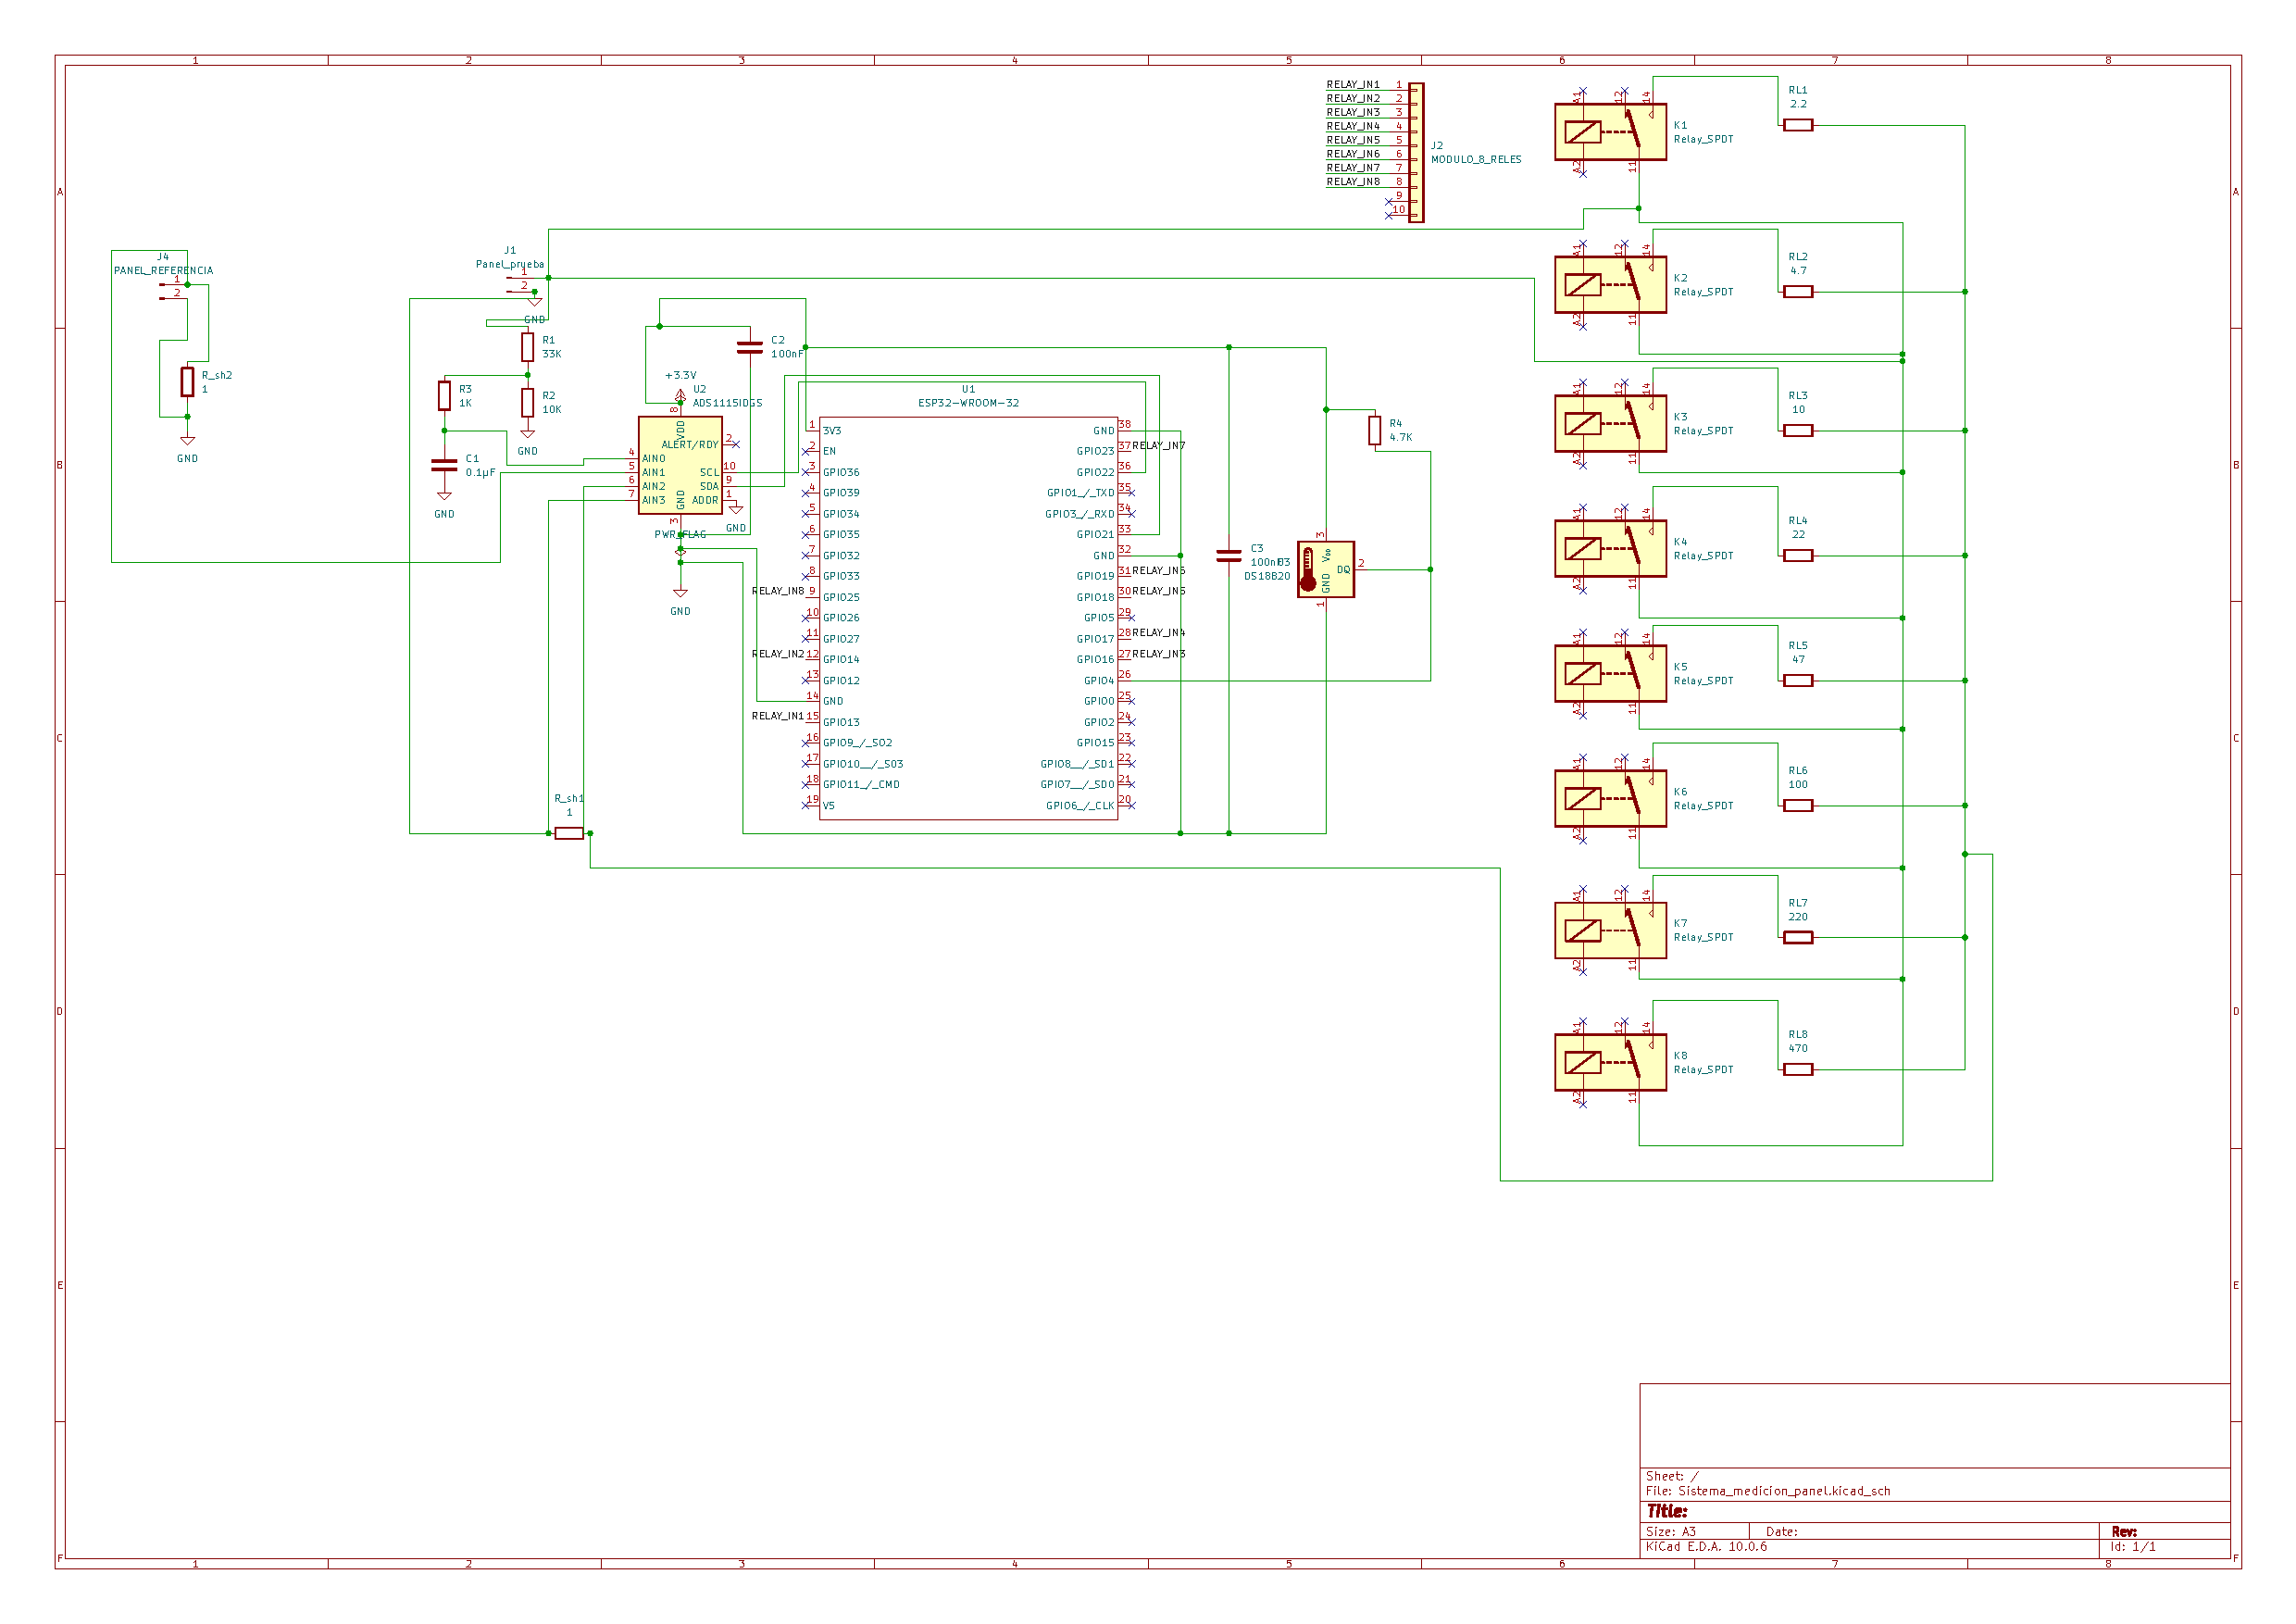
\includepdf[pages=1,fitpaper=true,pagecommand={\thispagestyle{empty}}]{Sistema_medicion_panel.pdf}
\end{document}
